\documentclass{report}

% ====== PACCHETTI DI BASE ======
\usepackage[utf8]{inputenc}
\usepackage[T1]{fontenc}
\usepackage[italian,english]{babel} % ultima lingua = principale
\usepackage{amsmath, amssymb, amsthm}
\usepackage{graphicx}
\usepackage{subcaption} 
\usepackage{booktabs}
\usepackage{float}
\usepackage{geometry}
\geometry{margin=2.5cm}
\usepackage[hidelinks]{hyperref}
\usepackage{tikz}
\usetikzlibrary{decorations.pathreplacing, positioning, arrows.meta}
% === Colored, numbered boxes for a thesis ===
\usepackage[most]{tcolorbox} % pacchetto principale
\tcbuselibrary{theorems,skins,breakable}
\usepackage{xcolor}

% Palette sobria (puoi modificare a piacere)
\definecolor{BoxFrame}{RGB}{60,60,60}   % bordo
\definecolor{BoxBack}{RGB}{245,245,245} % sfondo
\definecolor{Accent}{RGB}{128,0,32}    % accento per titoli

% Stile base riutilizzabile
\tcbset{
  thesisbox/.style={
    enhanced,
    breakable,               % va a capo sulle pagine
    colframe=BoxFrame,       % colore bordo
    colback=BoxBack,         % colore sfondo
    boxrule=0.6pt,           % spessore bordo
    arc=1.2mm,               % arrotondamento angoli
    left=6pt,right=6pt,top=6pt,bottom=6pt,
    title style={colback=white, colframe=BoxFrame},
    coltitle=Accent,
    fonttitle=\bfseries,
    attach boxed title to top left={yshift=-2mm, xshift=2mm},
    boxed title style={boxrule=0.6pt},
  },
}

% --- Versioni SENZA numerazione ---
\newtcolorbox{DefinitionBox}[1][]{thesisbox, title=Definition, #1}
\newtcolorbox{NoteBox}[1][]{thesisbox, title=Note, #1}
\newtcolorbox{ExampleBox}[1][]{thesisbox, title=Example, #1}

% --- Versioni CON numerazione in stile "Theorem-like" ---
% Numerate per capitolo (reset ogni \chapter); se usi \section come top-level, cambia "chapter" in "section"
\newtcbtheorem[number within=chapter]{Definition}{Definition}%
{thesisbox}{def}
\newtcbtheorem[number within=chapter]{Remark}{Note}%
{thesisbox}{rem}
\newtcbtheorem[number within=chapter]{Example}{Example}%
{thesisbox}{ex}

% ====== BIBLIOGRAFIA ======
\usepackage{csquotes}
\usepackage[backend=biber,style=numeric]{biblatex}
\addbibresource{bibliography.bib}

% ====== TITOLI GRANDI E NUMERAZIONE ======
\usepackage[explicit]{titlesec}

% --- Capitoli ---
\renewcommand{\chaptername}{}
\titleformat{\chapter}[hang]
  {\bfseries\Huge}
  {\thechapter\ }{0pt}{#1}
\titlespacing*{\chapter}{0pt}{-10pt}{20pt} 

% --- Sezioni ---
\titleformat{\section}[block]
  {\bfseries\LARGE}
  {\thesection}{1em}{#1}
\titlespacing*{\section}{0pt}{15pt}{10pt}

% --- Sottosezioni ---
\titleformat{\subsection}[block]
  {\bfseries\Large}
  {\thesubsection}{1em}{#1}
\titlespacing*{\subsection}{0pt}{10pt}{5pt}

% ====== FONT SIZE NORMALE PERSONALIZZATO ======
\makeatletter
\renewcommand\normalsize{%
   \@setfontsize\normalsize{13pt}{15.6pt}%
}
\makeatother



% ====== CODE LISTINGS (Python) ======
\usepackage{listings}

% Colori per il codice
\definecolor{codegray}{rgb}{0.45,0.45,0.45}
\definecolor{codepurple}{rgb}{0.58,0,0.82}
\definecolor{codeblue}{rgb}{0.10,0.10,0.70}
\definecolor{codebg}{rgb}{0.97,0.97,0.97}

% Stile Python per la tesi
\lstdefinestyle{pythonstyle}{
    backgroundcolor=\color{codebg},
    basicstyle=\ttfamily\small,
    keywordstyle=\color{codeblue}\bfseries,
    commentstyle=\color{codegray}\itshape,
    stringstyle=\color{codepurple},
    %numbers=left,
    %numberstyle=\tiny\color{codegray},
    stepnumber=1,
    numbersep=8pt,
    frame=single,
    rulecolor=\color{BoxFrame},
    breaklines=true,
    breakatwhitespace=false,
    showstringspaces=false,
    tabsize=4,
    captionpos=b
}

% Imposta Python come default (opzionale)
\lstset{style=pythonstyle, language=Python}






\begin{document}

% ====== FRONTESPIZIO ======
\begin{titlepage}
    \centering
    
\includegraphics[width=1\textwidth]{immagineuni.jpg}\par\vspace{1cm}
    {\scshape\Large Department of Physics\par}
    \vspace{1cm}
    {\scshape\Large Bachelor’s Degree in Physics\par}
    \vspace{2cm}
    {\huge\bfseries Simulation of LiteBIRD Instrumental Noise with the LBS Framework \par}
    \vspace{2cm}
    \begin{flushleft} 
        \large
        \textbf{Supervisor:} Prof. Maurizio Tomasi\\
    \end{flushleft}
    \vfill
    \begin{flushright}
        \large
        \textbf{Bachelor’s Thesis by:}\\
        Giulia Giommoni\\
        Student ID: 12201A
    \end{flushright}
    \vfill
    {\large Academic Year 2024--2025\par}
\end{titlepage}




% ====== ABSTRACT ======
\newpage
\section*{Abstract}
The study of Cosmic Microwave Background (CMB) anisotropies represents one of the most advanced frontiers of modern cosmology. The \textit{LiteBIRD} space mission aims to detect primordial B-modes, extremely weak polarized signals that would provide definitive evidence of cosmic inflation. However, achieving such sensitivity requires rigorous control of instrumental noise, particularly the low-frequency correlated component known as $1/f$ noise. This noise is especially critical because its temporal correlations project onto large angular scales (low multipoles $\ell$), where the B-mode signal exhibits its recombination peak, risking the masking of cosmological information.

This thesis work focuses on the modeling, implementation, and validation of efficient strategies for generating instrumental noise with the \textit{LiteBIRD Simulation (LBS)} framework. The central problem addressed is the computational management of large data volumes (Time-Ordered Data): the realistic simulation of a mission produces hundreds of millions of samples, making data allocation and processing a prohibitive task for standard memory resources.

To overcome this obstacle, two different noise generation functions operating in block-wise mode have been implemented and compared: 

\begin{enumerate}
    \item \texttt{add\_lbsNoise}: based on Fast Fourier Transform (FFT) algorithms already integrated into the LBS framework.
    \item \texttt{add\_OofaNoise}: based on the \texttt{ducc0} library, which uses recursive digital filters to transform white noise into $1/f$ noise in a continuous and computationally lightweight manner.
\end{enumerate}

The validation of the models was conducted through several analyses. Initially, in the time and frequency domains, the Power Spectral Density (PSD) was verified, confirming that both methods correctly reproduce the required knee frequency and spectral index. Subsequently, an optimized map-making pipeline using JIT compilation (Numba) was implemented to project an entire year of simulation onto the celestial sphere using HEALPix pixelization.

The resulting noise maps, limited to the intensity (temperature) component, allowed for the visualization of the characteristic stripping patterns induced by temporal correlations along the satellite's scanning strategy. Finally, the analysis in the harmonic domain of the angular power spectra ($C_\ell^{TT}$) confirmed the statistical consistency of the two models. The comparison highlights how the approach based on digital filters offers advantages in terms of temporal continuity between blocks and more efficient memory management.

In conclusion, this work provides a concrete tool for managing long-duration simulations. The results demonstrate that the block-wise approach allows for the processing of LiteBIRD's actual data volume.





% ====== INDICE ======
\tableofcontents
\newpage




% ====== CAPITOLI ======
\chapter{Introduction}

\section{Cosmic Microwave Background and Inflation}

The observation of the cosmic microwave background (CMB) temperature fluctuations has played a fundamental role in establishing the standard cosmological model, the $\Lambda$ cold dark matter ($\Lambda \mathrm{CDM}$) model, and in constraining key cosmological parameters and the large-scale properties of spacetime. While most of the information about the early Universe has historically been extracted from temperature anisotropies, the polarization of the CMB provides an additional and complementary source of information, offering access to physical processes that are otherwise difficult to probe \cite{2022}.

One of the most important open questions in modern cosmology concerns the origin of the primordial fluctuations that later evolved into the large-scale structure of the Universe. The leading theoretical framework addressing this question is cosmic inflation, a period of accelerated expansion occurring at very early times. During inflation, microscopic quantum fluctuations were stretched to macroscopic scales, seeding both density perturbations and tensor perturbations in the spacetime metric. These initial fluctuations eventually gave rise to galaxies, clusters, and the cosmic web observed today.

\begin{figure}[htbp]
    \centering
    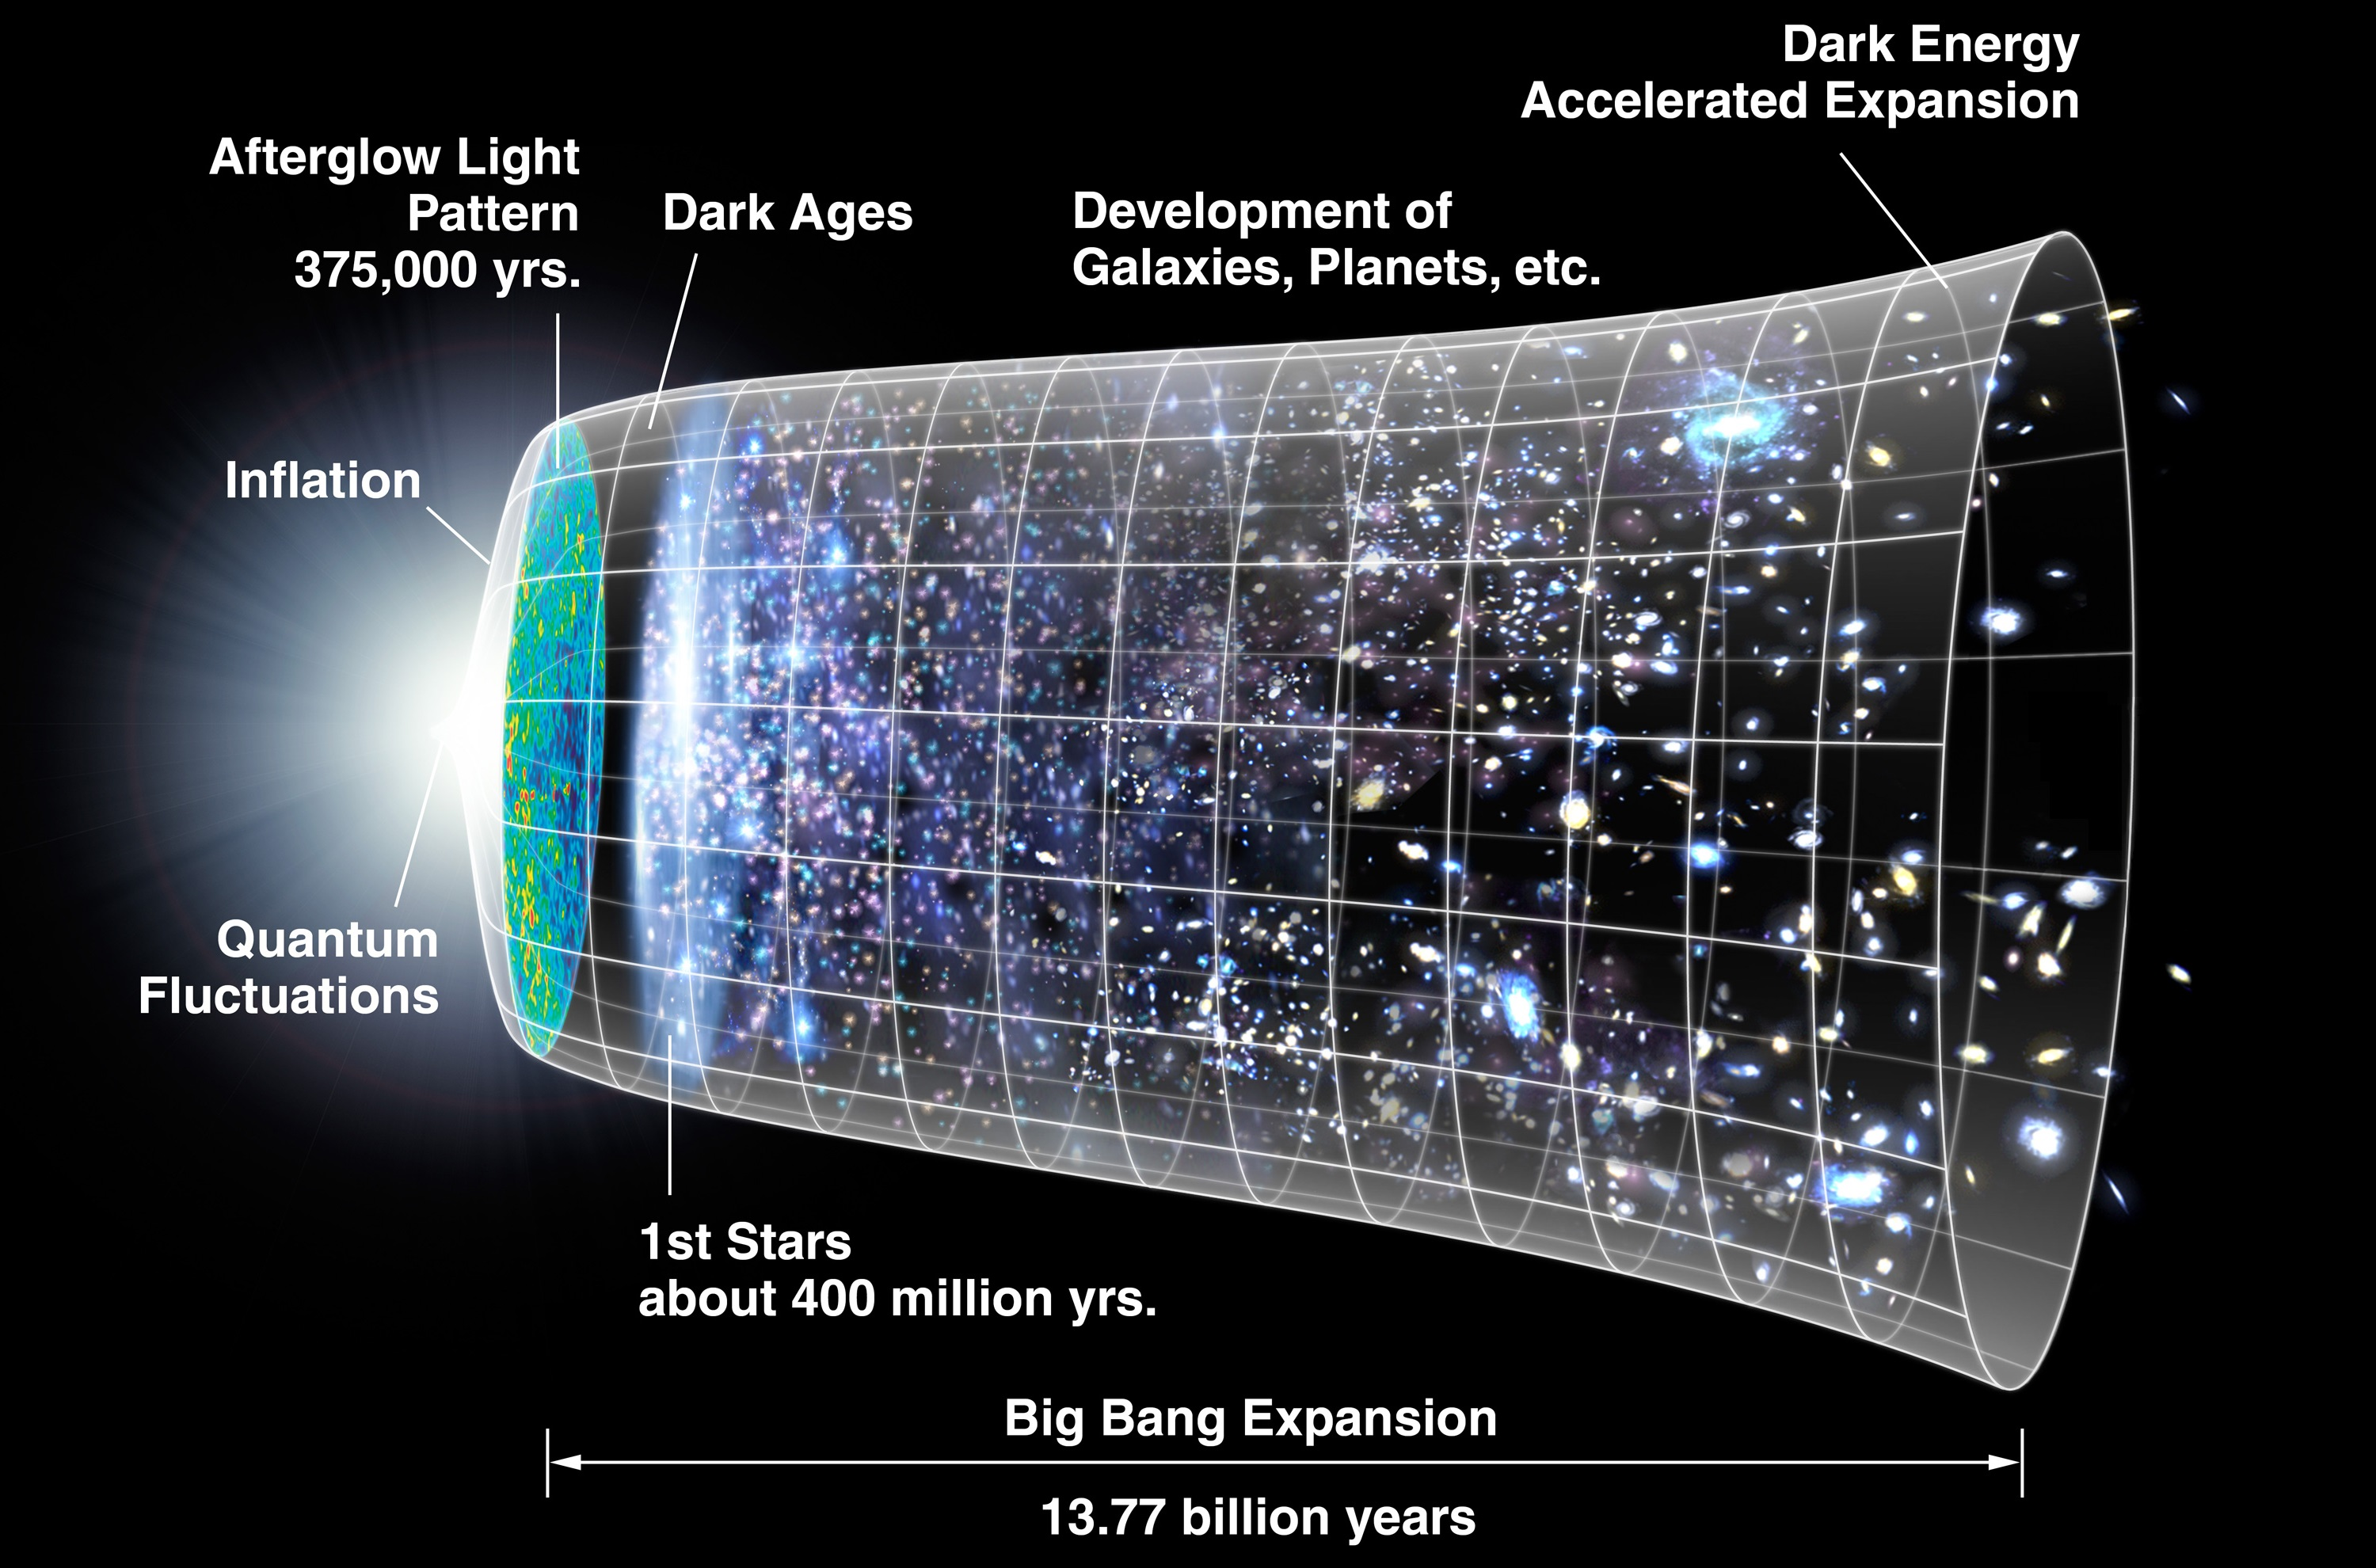
\includegraphics[width=0.7\textwidth]{1_bigbang_expansion}
    \caption{Timeline of the Universe according to the standard cosmological model. The diagram illustrates the expansion from the initial quantum fluctuations, through the epoch of inflation, to the emission of the CMB approximately 375,000 years after the Big Bang, and finally the subsequent formation of large-scale structures.}
    \label{fig:universe_timeline}
\end{figure}

Inflation predicts not only the scalar perturbations responsible for CMB temperature anisotropies, but also a stochastic background of primordial gravitational waves. While scalar perturbations dominate the temperature signal, tensor perturbations leave a characteristic imprint in the polarization of the CMB, providing a unique observational window onto the inflationary epoch. Detecting such a signal would offer direct evidence for inflation and allow access to energy scales far beyond the reach of terrestrial experiments \cite{2022}.



\section{CMB Polarization and Primordial \textit{B}-Modes}

The polarization of the CMB arises from Thomson scattering of photons in the presence of local quadrupole temperature anisotropies at the surface of last scattering and during the epoch of reionization. The polarization pattern on the sky can be decomposed into two components, known as \textit{E}-modes and \textit{B}-modes, which differ in their symmetry properties under parity transformations.

\textit{E}-mode polarization is primarily generated by scalar density perturbations and has been robustly detected by several experiments. \textit{B}-mode polarization, on the other hand, is of particular interest because it can be sourced by tensor perturbations, such as primordial gravitational waves produced during inflation. Since scalar perturbations do not generate \textit{B}-modes at linear order, the detection of a primordial \textit{B}-mode signal would constitute a distinctive signature of inflationary physics.

\begin{figure}[htbp]
    \centering
    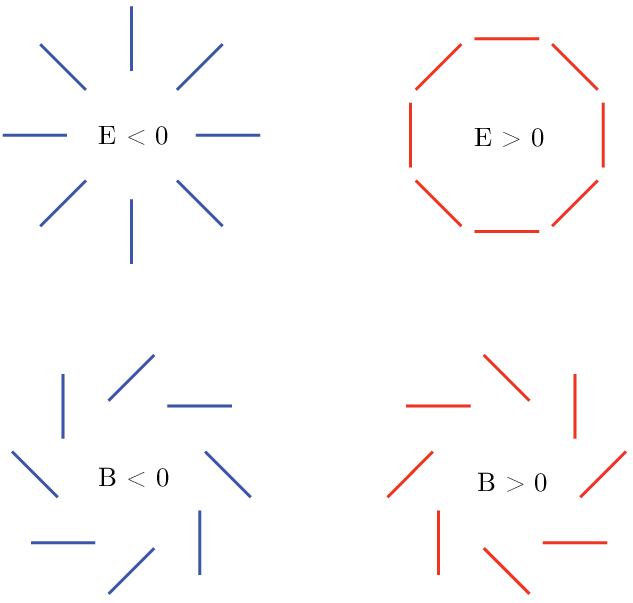
\includegraphics[width=0.38\textwidth]{1_eb_modes.png}
    \caption{Schematic representation of CMB polarization modes. Top: $E$-modes exhibit a curl-free, symmetric pattern under parity transformation ($E > 0$ for tangential, $E < 0$ for radial). Bottom: $B$-modes exhibit a divergence-free, spiral pattern, changing sign under parity reflection.}
    \label{fig:eb_modes}
\end{figure}

In addition to a possible primordial contribution, \textit{B}-modes can also be generated through secondary effects. Gravitational lensing by large-scale structures distorts the polarization field, converting part of the \textit{E}-mode signal into \textit{B}-modes, while Galactic foreground emissions further contaminate the observed signal. Disentangling the primordial component therefore requires high sensitivity, broad frequency coverage, and careful control of instrumental and observational systematics.



\section{The LiteBIRD Mission}

\textit{LiteBIRD (Lite \textit{B}-mode polarization and Inflation from cosmic background Radiation Detection)} is a space mission dedicated to primordial cosmology and fundamental physics. Its primary scientific goal is the detection of polarization from primordial gravitational waves, which would provide direct evidence for cosmic inflation and probe physics at energy scales far beyond those accessible on Earth \cite{2022}.

LiteBIRD will operate at the Sun--Earth Lagrange point L2, a stable environment that enables continuous full-sky observations with minimal contamination from the Earth, Moon, and Sun. From this orbit, the satellite will survey the CMB polarization over a nominal mission duration of three years.

The mission observes the sky in 15 frequency bands from 34 to 448~GHz, allowing efficient separation of the primordial CMB signal from Galactic and extragalactic foregrounds. LiteBIRD aims for an unprecedented total sensitivity of approximately 
$2.2~\mu\mathrm{K \cdot arcmin}$, with a typical angular resolution of about 
$0.5^\circ$ at 100~GHz, as reported in \cite{2022}. This makes it complementary to ground-based experiments, which generally target smaller sky areas, whereas LiteBIRD focuses on the largest angular scales through full-sky coverage.

A key scientific requirement is to reach a sensitivity sufficient to detect the primordial gravitational wave amplitude, expressed in terms of the tensor-to-scalar ratio $r$\footnote{
The tensor-to-scalar ratio $r$ quantifies the relative amplitude of primordial tensor perturbations (gravitational waves) with respect to scalar perturbations (density fluctuations) generated during inflation. It is defined as the ratio between the power spectra of tensor and scalar modes,
\[
r \equiv \frac{\Delta_h^2(k)}{\Delta_\zeta^2(k)} = \frac{A_t}{A_s},
\]
where $\Delta_h^2(k)$ and $\Delta_\zeta^2(k)$ denote the dimensionless tensor and scalar power spectra, and $A_t$ and $A_s$ are their corresponding amplitudes evaluated at a given pivot scale $k$. A detection of a non-zero value of $r$ would provide direct evidence for primordial gravitational waves and strongly support the inflationary paradigm.
}. LiteBIRD aims for a total uncertainty $\delta r < 10^{-3}$, enabling either detection of primordial \textit{B}-modes or stringent constraints on inflationary models. In particular, it targets both the recombination peak ($\ell \simeq 80$) and the reionization peak ($\ell \lesssim 10$) in the \textit{B}-mode power spectrum, which together would provide robust evidence for an inflationary origin.

\begin{figure}[htbp]
    \centering
    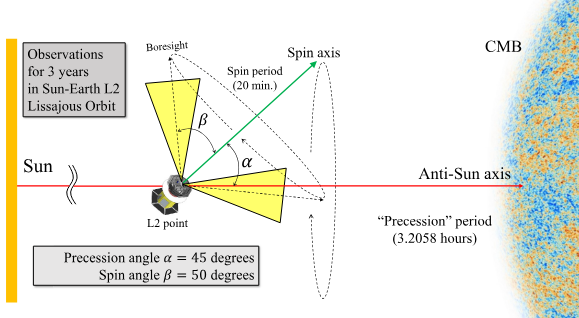
\includegraphics[width=0.8\textwidth]{1_satellite.png}
    \caption{The telescope boresight is at an angle $\beta = 50^{\circ}$ to the spin axis and rotates at a rate of $0.05$\,rpm. The spin axis is rotated around the anti-Sun direction through precession with an angle $\alpha = 45^{\circ}$ in $3.2058$\,h. The anti-Sun axis rotates around the Sun in one year. With a combination of the three motions, the boresight can cover the entire sky in half a year. (Image adapted from \cite{2022}).}
    \label{fig:litebird_scan}
\end{figure}

The payload comprises three telescopes covering complementary frequency ranges: the Low-Frequency Telescope (LFT), the Mid-Frequency Telescope (MFT), and the High-Frequency Telescope (HFT). Multichroic detectors allow each pixel to observe multiple frequency bands, maximizing sensitivity while keeping the focal plane compact.

LiteBIRD scans the sky using a combination of continuous rotation around its own axis, slow precession around the Sun–Earth direction, and annual revolution around the Sun. This scanning strategy ensures uniform sky coverage, high redundancy in polarization angle sampling, and suppression of systematic effects. A continuously rotating half-wave plate modulates the polarization signal, reducing low-frequency ($1/f$) noise and instrumental systematics. Thermal and mechanical stability of the spacecraft further minimize noise contributions.

Access to the largest angular scales, particularly the reionization \textit{B}-mode signal, is uniquely achievable from space. Correlated low-frequency noise and long-term drifts can significantly affect these measurements, making accurate instrumental noise modeling critical for assessing LiteBIRD's sensitivity and scientific performance.



\section{Aim and Structure of the Thesis}
The main objective of this thesis is the simulation and comparison of instrumental noise models for the LiteBIRD mission, focusing on white noise and correlated $1/f$ noise, which dominate in large-angular-scale CMB polarization experiments.

The work uses the LiteBIRD Simulation Framework (LBS), a Python-based simulation 
package for modeling the data acquisition of LiteBIRD instruments, as presented 
in \cite{Tomasi2025}, along with the \texttt{ducc0} numerical library\footnote{\url{https://gitlab.mpcdf.mpg.de/mtr/ducc}} 
by Martin Reinecke for efficient numerical computation. In this work, two new noise-addition functions have been implemented to operate 
block-wise, enabling long-duration simulations while controlling memory usage. 
These functions are based on pre-existing noise-generation routines: one provided by the LiteBIRD Simulation Framework and one by the \texttt{ducc0} library.

The two noise models are validated and compared in both time and frequency domains. Time-domain signals and power spectral densities are examined to verify agreement with theoretical expectations, while noise-only sky maps and hit maps assess the impact of correlated noise on large angular scales. Performance is also evaluated in terms of computational time and memory usage, with attention to optimization strategies for long-term simulations.

This thesis is organized as follows. Chapter~2 provides the scientific background on instrumental noise in CMB experiments, detailing white and $1/f$ noise, power spectral density, and HEALPix sky pixelization. Chapter~3 describes the simulation framework, the scanning strategy, and the detector models adopted for LiteBIRD. Chapter~4 presents the noise generation strategy and the technical implementation of the two block-wise models. Chapter~5 focuses on the validation of the models through time-domain and frequency-domain analyses. Chapter~6 extends the analysis to long-term simulations, map-making, and the estimation of the angular power spectrum for temperature ($C_\ell^{TT}$). Finally, Chapter~7 summarizes the results obtained and discusses potential future developments.

\chapter{Scientific Background}


\section{CMB Observables and the Role of Instrumental Noise}

The LiteBIRD satellite is designed to measure the anisotropies of the Cosmic Microwave Background (CMB) through the three relevant Stokes parameters: the temperature anisotropy $T$, the linear polarization components $Q$ (horizontal/vertical) and $U$ (diagonal).

LiteBIRD detectors do not measure temperature directly; instead, they measure the radiative intensity (or absorbed power) of the incoming electromagnetic radiation, integrated over finite frequency bands and for specific polarization states. From the measured intensity and intensity differences, the Stokes parameters $I, Q,$ and $U$ are reconstructed. In the context of CMB observations, the total intensity $I$ is conventionally expressed as a temperature anisotropy $T$.

Since the CMB temperature fluctuations are very small compared to the mean CMB temperature $T_{\mathrm{CMB}} \simeq 2.725\,\mathrm{K}$, the conversion from intensity to temperature is performed using the linearized Planck law. For a given frequency $\nu$, the relation between intensity fluctuations $\Delta I_\nu$ and temperature fluctuations $\Delta T$ is
\begin{equation}
\Delta I_\nu =
\left.\frac{dB_\nu(T)}{dT}\right|_{T=T_{\mathrm{CMB}}} \Delta T ,
\end{equation}
where $B_\nu(T)$ is the Planck blackbody spectrum,
\begin{equation}
B_\nu(T) = \frac{2 h \nu^3}{c^2} \frac{1}{e^{h\nu/(k_B T)} - 1}.
\end{equation}
Using this relation, the measured intensity fluctuations are converted into maps of $T, Q,$ and $U$, which are typically expressed in units of $\mu\mathrm{K}_{\mathrm{CMB}}$.

Each of the resulting sky maps $X(\hat{n}) = \{T(\hat{n}), Q(\hat{n}), U(\hat{n})\}$ can be expanded in spherical harmonics. For the temperature field, the expansion reads
\begin{equation}
T(\hat{n}) = \sum_{\ell=0}^{\infty} \sum_{m=-\ell}^{\ell} a^{T}_{\ell m} \, Y_{\ell m}(\hat{n}) .
\end{equation}

The linear polarization fields $Q(\hat{n})$ and $U(\hat{n})$ are not scalar quantities, but components of a spin-2 field on the sphere. For this reason, they are conveniently combined into the complex quantities $Q(\hat{n}) \pm iU(\hat{n})$, which can be expanded in terms of spin-weighted spherical harmonics:
\begin{equation}
Q(\hat{n}) \pm iU(\hat{n}) =
\sum_{\ell=2}^{\infty} \sum_{m=-\ell}^{\ell}
\left( a^{E}_{\ell m} \pm i a^{B}_{\ell m} \right)
\, {}_{\pm 2}Y_{\ell m}(\hat{n}) .
\end{equation}
This decomposition naturally defines the scalar E-mode and B-mode polarization components.

From the harmonic coefficients $a^{X}_{\ell m}$, the angular power spectra are defined as
\begin{equation}
C_\ell^{XY} = \frac{1}{2\ell + 1} \sum_{m=-\ell}^{\ell}
\left\langle a^{X}_{\ell m} \, a^{Y*}_{\ell m} \right\rangle ,
\end{equation}
where $X,Y \in \{T,E,B\}$. In particular, the $C_\ell^{BB}$ power spectrum quantifies the amount of B-mode polarization as a function of the multipole $\ell$, corresponding to different angular scales on the sky.

\begin{figure}[htbp]
    \centering
    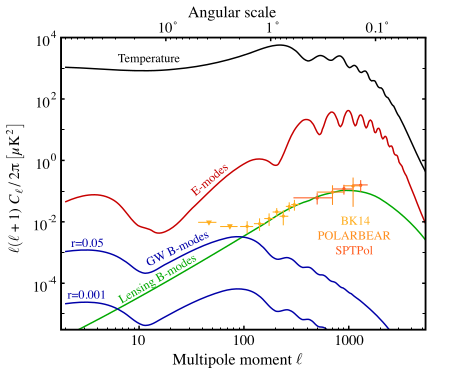
\includegraphics[width=0.68\textwidth]{2_theory_spectra.png}
    \caption{Theoretical predictions for CMB temperature, $E$-mode, and $B$-mode polarization power spectra. The plot highlights the faintness of the primordial $B$-mode signal (blue curves for different values of $r$) compared to the lensing-induced $B$-modes (green) and the dominant temperature anisotropies.}
    \label{fig:theory_spectra}
\end{figure}

The reconstruction of the CMB temperature and polarization fields does not start from direct sky maps, but from TOD streams produced by the detectors as the instrument scans the sky. Each detector sample corresponds to a measurement at a given time, pointing direction, and polarization orientation, and can be modeled as the sum of a sky signal and an instrumental noise contribution.

For a polarized detector observing the sky at time \( t \), the measured signal can be written schematically as
\begin{equation}
y_t = I_p + Q_p \cos(2\psi_t) + U_p \sin(2\psi_t) + n_t ,
\end{equation}
where \( I_p, Q_p, U_p \) are the Stokes parameters of the sky pixel \( p \), \( \psi_t \) is the detector polarization angle, and \( n_t \) denotes the instrumental noise. This relation can be compactly expressed in matrix form as
\begin{equation}
y = Ax + n,
\end{equation}
where \( y \) contains the TOD samples, \( x \) represents the pixelized sky map, \( A \) is the pointing matrix, and \( n \) is the noise vector \cite{Tegmark2001,Ashdown2007}.

In CMB experiments, each sky pixel is observed multiple times with different detector orientations, allowing the sky signal to be reconstructed from the redundant measurements. The statistical properties of the instrumental noise determine how individual samples are combined in the final map.

In realistic observations, however, instrumental noise is not purely uncorrelated. While part of the noise can be approximated as white, a significant fraction exhibits long-range temporal correlations associated with low-frequency instabilities in the detectors and readout system. If not properly modeled and mitigated, correlated noise can introduce large-scale artifacts in the reconstructed maps, posing a major challenge for polarization experiments targeting the large angular scales relevant for B-mode measurements.

The statistical properties of instrumental noise are conveniently described in the frequency domain through its power spectral density (PSD), which characterizes its temporal correlations \cite{Ashdown2007}. In particular, low-frequency noise components can couple at large angular scales in the sky through the scanning strategy, leading to excess power at low multipoles if not properly considered. For this reason, an accurate modeling of instrumental noise are essential for CMB experiments such as LiteBIRD, whose primary scientific goal is the measurement of the extremely weak B-mode polarization signal.

An important aspect of low-frequency instrumental noise is that its impact on the reconstructed maps is not easily distinguishable from cosmological signals. Because CMB observations are obtained from TOD through a scanning strategy, temporal fluctuations in the detector output are mapped onto angular fluctuations on the sky. In particular, noise components that vary slowly in time correspond to structures that are coherent over large angular scales. In harmonic space, these large-scale features project onto low multipoles $\ell$, the same regime where the primordial CMB signal carries most of its information. As a result, correlated low-frequency noise can mimic true cosmological anisotropies at low $\ell$, rather than simply adding random fluctuations. This degeneracy between instrumental noise and sky signal makes the control and mitigation of low-frequency noise a critical requirement for experiments such as LiteBIRD, which aim to measure extremely weak B-mode polarization on large angular scales.




\section{White Noise and $1/f$ Noise}

The output of any detector inevitably contains statistical noise, which limits the sensitivity of the measurements. Instrumental noise can be classified into two main components: uncorrelated (white) noise and correlated ($1/f$) noise. Each type of noise affects the measurement in different ways and must be properly characterized to understand its impact on the reconstructed sky maps.

\begin{figure}[htbp]
     \centering
     \begin{subfigure}[b]{0.38\textwidth}
         \centering
         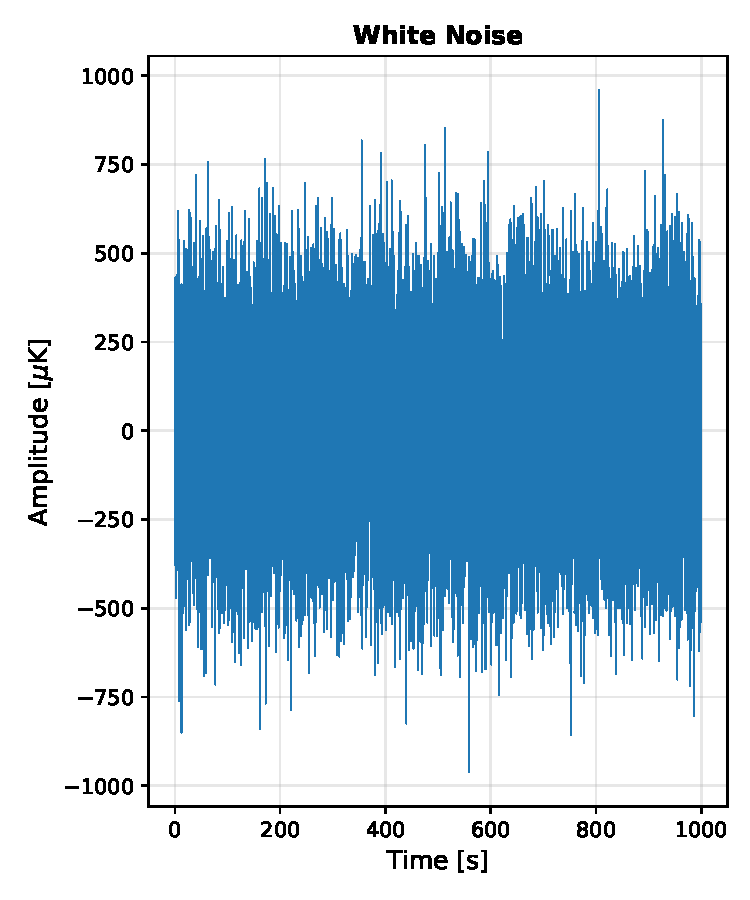
\includegraphics[width=\textwidth]{2_white.pdf}
         \label{fig:white_noise}
     \end{subfigure}
     \hspace{3mm} 
     \begin{subfigure}[b]{0.38\textwidth}
         \centering
         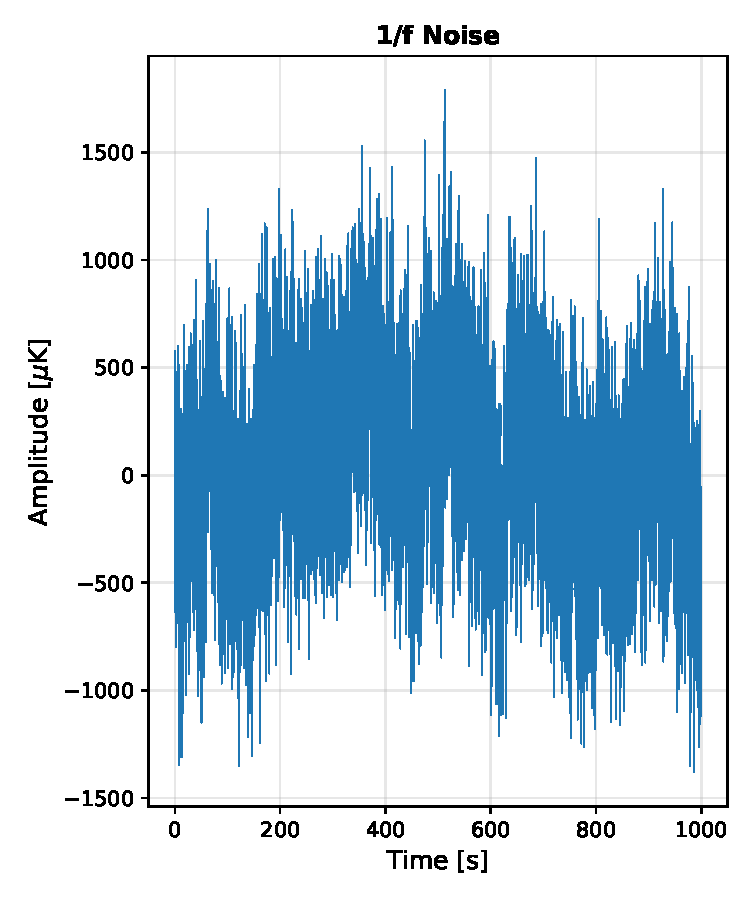
\includegraphics[width=\textwidth]{2_1overf.pdf}
         \label{fig:one_over_f}
     \end{subfigure}
     \caption{Comparison of noise realizations in the time domain. Left: White Gaussian noise, characterized by independent samples and a flat spectrum. Right: Correlated $1/f$ noise, showing slow low-frequency drifts that can be misinterpreted as large-scale cosmological signals.}
     \label{fig:noise_comparison}
\end{figure}

\subsection{White Noise}
White noise is a stochastic process with a flat power spectral density (PSD), meaning that all temporal frequencies contribute equally to the signal. In discrete time, white noise can be represented as a sequence of statistically independent random variables with zero mean and finite variance. If the samples are normally distributed, the noise is referred to as additive white Gaussian noise.

Mathematically, white noise satisfies
\begin{equation}
\langle n(t) \rangle = 0, \qquad
\langle n(t)n(t') \rangle = \sigma^2 \delta(t-t'),
\end{equation}
where $\sigma^2$ is the white noise level. Its PSD is therefore constant over frequency:
\begin{equation}
P(f) = \sigma^2.
\end{equation}

Two key properties of white noise are:
\begin{enumerate}
    \item Flat spectrum: all frequencies contribute equally to the signal power.
    \item No temporal correlation: samples at different times are statistically independent.
\end{enumerate}

It is important to note that Gaussianity and whiteness are distinct concepts. Gaussianity refers to the probability distribution of the signal amplitude, while whiteness refers to the distribution of power across frequencies. A signal can be Gaussian but not white, or white but not Gaussian.


\subsection{1/f Noise}
$1/f$ noise, also known as pink noise, is a low-frequency correlated component, commonly observed in microwave detectors and radio receivers. Unlike white noise, $1/f$ noise exhibits long-term correlations, causing slow drifts in the detector output. Its PSD follows an approximate power-law behavior:
\begin{equation}
P(f) = \sigma^2 \left(\frac{f_{knee}}{f}\right)^\alpha,
\end{equation}
where $f_{knee}$ is the knee frequency, $\alpha$ is the spectral index (typically between 1 and 2), and $\sigma^2$ is the white noise level. Below $f_{knee}$, the $1/f$ component dominates, while above $f_{knee}$ the noise becomes effectively white. This behavior introduces excess power at low frequencies, which projects onto large angular scales in sky maps and can significantly affect B-mode polarization measurements.

In practical terms, $1/f$ noise arises from slow instabilities in the detector or the readout electronics, often related to thermal or electronic fluctuations. Its presence motivates the use of stable cryogenic systems and careful calibration to minimize drifts and gain fluctuations.

In summary, white noise contributes equally at all temporal frequencies and is uncorrelated over time, while $1/f$ noise dominates at low frequencies and exhibits long-term correlations. Understanding the statistical differences between these two noise components is essential for designing realistic simulations of time-ordered data and for predicting their impact on the reconstructed sky maps.





\section{Power Spectral Density}

The power spectral density (PSD) describes how the power of a signal is distributed across frequencies. In CMB studies, it is a fundamental tool to characterize instrumental noise. The PSD provides insight into the frequency-dependent behavior of the noise.


\subsection{PSD Estimation with the FFT}
A simple approach to estimate the PSD is based on the discrete Fourier transform (DFT) of a sampled signal \cite{press2007numerical}. For a time series sampled at $N$ points $c_0, \dots, c_{N-1}$, the DFT is

\begin{equation}
C_k = \sum_{j=0}^{N-1} c_j \, e^{2\pi i jk / N}, \quad k = 0, \dots, N-1.
\end{equation}

The periodogram estimates the PSD as the squared modulus of the DFT:

\begin{equation}
P(f_k) = \frac{1}{N^2} |C_k|^2, \quad k = 0, \dots, \frac{N}{2}.
\end{equation}

This gives the power associated with positive frequencies $f_k = k / (N \Delta)$, where $\Delta$ is the sampling interval. While straightforward, the periodogram suffers from spectral leakage, where power from one frequency spreads into neighboring bins. Leakage arises because a finite-length segment of data is effectively multiplied by a square window in time, whose Fourier transform contains high-frequency components.

To reduce leakage, each data segment can be multiplied by a window function $w_j$ that smoothly rises and falls at the segment edges. The resulting windowed periodogram is

\begin{equation}
D_k = \sum_{j=0}^{N-1} c_j w_j \, e^{2\pi i jk / N}, \quad
P(f_k) = \frac{1}{\sum_j w_j^2} |D_k|^2.
\end{equation}

Common windows include Hann, Hamming, and Bartlett. Windowing suppresses leakage but slightly increases the variance of the PSD estimate, since data near the edges are down-weighted \cite{press2007numerical}.


\subsection{Welch's Method}

Welch's method improves the PSD estimate by splitting the signal into overlapping segments, applying a window to each, computing their periodograms, and averaging them. This approach reduces variance compared to the simple periodogram and maintains low leakage. Typical overlap is 50\% of the segment length.

The main steps of Welch's method are:

\begin{enumerate}
    \item Segmenting the signal: the signal is divided into partially overlapping segments to increase the number of independent estimates.
    \item Windowing: each segment is multiplied by a window function (e.g., Hann or Hamming) to reduce edge effects. The window suppresses spectral leakage, i.e., the spreading of power from a frequency to neighboring frequencies.
    \item Fourier Transform: the FFT of each windowed segment is computed.
    \item Power computation: the local periodogram of each segment is obtained as the squared modulus of the FFT.
    \item Averaging: the periodograms of all segments are averaged to obtain the final PSD.
    \begin{itemize}
        \item Averaging reduces the variance of the estimate, smoothing fluctuations around the mean.
        \item As a side effect, the frequency resolution is reduced.
    \end{itemize}
\end{enumerate}

In Python, \texttt{scipy.signal.welch()} performs these steps efficiently, taking a time series and returning its PSD.

When a segment of the signal is treated as zero outside its boundaries, the FFT of the segment corresponds to the Fourier transform of the signal multiplied by a characteristic function $\chi$, which results in a frequency spread around the central frequency $\nu_0$ instead of a Dirac delta. By multiplying the segment by a window function, the resulting PSD is effectively the convolution of the signal's Fourier transform with the Fourier transform of the window. This softens the spectral distribution and further reduces leakage, providing a more accurate estimate of the PSD.

The PSD obtained in this way quantifies the power in each frequency band, which is essential for analyzing instrumental noise in CMB simulations.





\section{HEALPix Sky Pixelization}

Many experiments in observational cosmology, and in particular studies of the Cosmic Microwave Background (CMB), produce data that naturally live on the surface of a sphere. In order to analyze such data numerically, it is necessary to introduce a discretized representation of the sky, i.e., a pixelization of the sphere.

A pixelization scheme widely adopted in CMB data analysis is HEALPix, short for \textit{Hierarchical Equal Area isoLatitude Pixelization} of the sphere, introduced by Górski et al.~\cite{Gorski2005}. HEALPix was specifically designed to meet the requirements of full-sky cosmological observations and has become a standard tool in modern CMB experiments.

The HEALPix scheme is characterized by three key features:

\begin{itemize}
    \item Equal-area pixels, ensuring that each pixel covers the same solid angle on the sky. This property prevents spatial variations in noise level due solely to the pixelization and guarantees that white instrumental noise remains white after projection into map space.
    \item Hierarchical structure, which allows the sky resolution to be increased by recursively subdividing pixels. This is particularly advantageous for handling large data sets and enables efficient memory management and multiresolution analyses.
    \item Iso-latitude pixel centers, meaning that pixels are arranged in rings of constant latitude. This feature is crucial for enabling fast spherical harmonic transforms, which are central to CMB data analysis.
\end{itemize}

\begin{figure}[htbp]
    \centering
    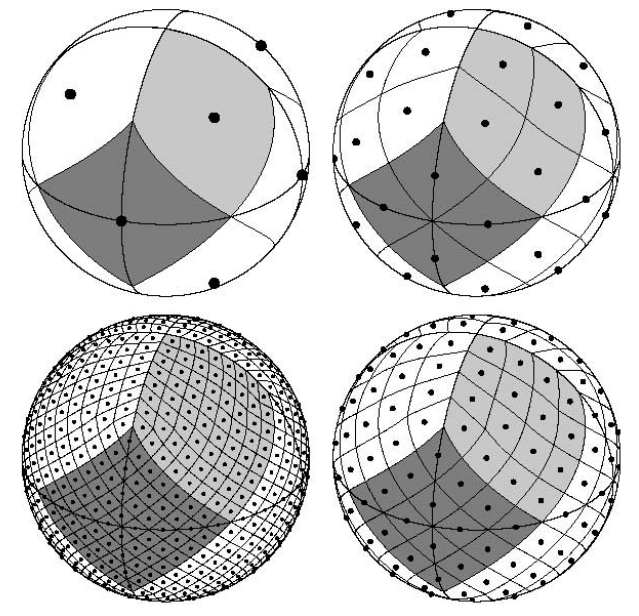
\includegraphics[width=0.45\textwidth]{2_healpix.png}
    \caption[Orthographic view of the HEALPix partition]{Orthographic view of the HEALPix partition of the sphere. The sequence illustrates the hierarchical subdivision of the 12 base-resolution pixels as the resolution parameter $N_{side}$ increases ($N_{side} = 1, 2, 4, 8$), maintaining equal-area properties for all pixels. Image taken from \cite{Gorski2005}.}
    \label{fig:healpix_hierarchy}
\end{figure}

At the lowest resolution, HEALPix divides the sphere into 12 base pixels of equal area. This base tessellation is constructed by partitioning the sphere into 3 regions in latitude: a northern polar cap, an equatorial region, and a southern polar cap. Each of these regions is further divided into 4 pixels in longitude, resulting in a total of $3 \times 4 = 12$ base pixels.

The resolution of a HEALPix map is controlled by a single integer parameter, \texttt{Nside}, which specifies how many times each side of a base pixel is subdivided. Increasing \texttt{Nside} increases the angular resolution of the map while preserving the equal-area and hierarchical properties of the pixelization.

The total number of pixels in a HEALPix map is given by:
\begin{equation}
N_{\text{pix}} = 12\,N_{\text{side}}^{2}.
\end{equation}

Each pixel covers the same solid angle:
\begin{equation}
\Omega_{\text{pix}} = \frac{4\pi}{N_{\text{pix}}} = \frac{\pi}{3\,N_{\text{side}}^{2}}.
\end{equation}

Practical applications require choosing an appropriate value of \texttt{Nside}. Increasing the resolution improves angular fidelity but also leads to: higher memory usage, longer computation times, larger time-ordered and map-level data products.

\chapter{Simulation Framework and Instrument Modeling}


\section{The LiteBIRD Simulation Framework}

The \textit{LiteBIRD Simulation Framework (LBS)} is a Python-based library designed to model the data acquisition process of the LiteBIRD instruments and to simulate the time-ordered data (TOD) that will be produced once the satellite is deployed in space. The primary motivation behind LBS is to validate the instrument design and assess whether the mission can achieve its main scientific goal, namely setting a stringent upper limit on the tensor-to-scalar ratio $r$, under the assumption of a fiducial model with $r = 0$ \cite{Tomasi2025}.

LBS has been developed to support end-to-end (E2E) simulations, which typically include:
\begin{enumerate}
    \item the generation of a model sky signal;
    \item the simulation of the spacecraft motion and instrument response;
    \item the production of detector timelines (TOD);
    \item the reconstruction of sky maps at multiple frequencies;
    \item the estimation of angular power spectra and cosmological parameters.
\end{enumerate}

Rather than implementing a single monolithic E2E pipeline, the LiteBIRD collaboration adopted a modular framework approach. LBS provides a collection of independent modules that can be combined to build different simulation pipelines, depending on the scientific objective.

This design offers several advantages:
\begin{itemize}
    \item multiple pipelines can be developed consistently, including full E2E simulations, simplified pipelines for rapid testing, and dedicated pipelines targeting specific effects;
    \item the reuse of common modules ensures consistency in the mathematical models describing the instrument and in the data formats used across different simulations;
    \item individual components, such as noise models or scanning strategies, can be modified or replaced without affecting the rest of the pipeline.
\end{itemize}

These features make LBS particularly suitable for controlled studies of instrumental effects, such as the analysis of different noise-generation techniques presented in this thesis.


\section{Simulation Architecture and Pipeline Structure}
The core component of LBS is the \texttt{Simulation} class, which represents the central container of any simulation pipeline built within the framework. This class manages the global configuration of the simulation and coordinates the interaction between the various modules, such as scanning strategy, instrument modeling, TOD allocation, and noise generation.

Several key pieces of information are shared across different modules through the \texttt{Simulation} object. For instance, the duration of the simulation determines both the total number of time samples to be allocated in memory and the temporal evolution of the spacecraft pointing. Similarly, the initialization of a random number generator ensures reproducibility across simulations.

The \texttt{Simulation} class also provides access to the Instrument Model database, allowing instrument and detector parameters to be loaded in a consistent and transparent way.



\section{Observation Model: Time-Ordered Data and Pointing}

A central concept in LBS is the \textit{Time-Ordered Data (TOD)}, which represent the output timelines of the detectors and are stored as sequences of samples acquired at a fixed sampling rate. In general, the TOD can be arranged in a two-dimensional matrix of size $N \times M$, where $N$ is the number of detectors and $M$ is the number of time samples.

In addition to the detector timelines, simulations require accurate pointing information, which specifies both the sky direction observed by each detector and its orientation with respect to the local reference frame. At each time sample, the pointing is fully described by three angles.

The direction of observation is encoded by the spherical coordinates $(\theta, \varphi)$, where $\theta$ is the colatitude (defined as $90^\circ$ minus the latitude) and $\varphi$ is the longitude. The detector orientation is instead described by a polarization angle $\phi$, defined with respect to the local meridian or parallel at the observed sky position. This angle specifies the direction of maximum sensitivity to linearly polarized radiation.

In this work, the pointing information associated with each detector therefore consists of:
\begin{itemize}
    \item two angles $(\theta, \varphi)$ describing the direction of the main beam on the sky;
    \item a single effective polarization angle $\phi$.
\end{itemize}

The effective polarization angle includes the contribution from both the intrinsic detector orientation and the rotation of the \textit{Half-Wave Plate (HWP)}. The HWP is a birefringent optical element, typically realized using materials such as sapphire, whose thickness is chosen to introduce a phase shift of half a wavelength ($\lambda/2$) between orthogonal polarization components.

By rotating continuously during the observation, the HWP modulates the polarized component of the incoming radiation. This modulation shifts the polarization signal to higher temporal frequencies, reducing the impact of correlated low-frequency ($1/f$) noise and instrumental systematic effects. Although this leads to a more complex time-domain signal, it significantly improves the robustness of the polarization measurement.




\section{Scanning Strategy}

The scanning strategy describes how the spacecraft surveys the sky as a function of time and plays a crucial role in determining the structure of the TOD and the impact of correlated noise.

LiteBIRD will perform a continuous sky survey, achieved through a combination of periodic rotations rather than discrete pointings. In particular, the spacecraft motion can be described as the composition of three rotations:
\begin{itemize}
    \item a rotation around the spacecraft spin axis at constant angular speed;
    \item a precession of the spin axis around the Sun–Earth direction;
    \item the annual motion of the Sun–Earth axis around the Sun.
\end{itemize}

LBS models this scanning strategy by encoding the spacecraft rotations using quaternions. To improve computational efficiency, the quaternions are sampled at a frequency lower than the detector sampling rate and then interpolated to the nominal rate using spherical linear interpolation.

In this thesis, both IMo-based scanning strategies, derived from the official Instrument Model, and simplified scanning setups are employed. The latter are particularly useful for testing and validation purposes, as they reduce complexity and allow the isolation of specific effects related to instrumental noise.


\section{Instrument and Detector Modeling}

Any realistic simulation requires a detailed description of how the instrument is built and how it operates. In the LiteBIRD context, this information is provided by the Instrument Model (IMo), a structured database containing the calibrated and measured parameters describing the spacecraft, the optical system, and the individual detectors.



\subsection{The Instrument Model (IMo)}
The \textit{Instrument Model (IMo)} is the collection of all the design parameters of the 
LiteBIRD instrument, telescope, and spacecraft. It describes the nominal configuration of the mission, including the spacecraft layout, the optical system, and the focal plane design. Each quantity in the IMo is referenced through a hierarchical path and a version identifier, ensuring traceability and 
reproducibility of simulations.

Within LBS, the IMo is accessed through structured objects representing different entities, such as:
\begin{itemize}
    \item \texttt{scanning\_parameters}, defining the nominal scanning strategy;
    \item \texttt{instrument\_info}, describing global properties of the focal plane;
    \item \texttt{detector\_info}, containing noise and sampling characteristics of individual detectors;
    \item \texttt{channel\_info}, providing average properties for detectors operating at the same frequency.
\end{itemize}

LBS allows simulations to be configured either using the official LiteBIRD IMo or a reduced, publicly accessible version containing synthetic but representative parameters. The latter is particularly useful for development and testing purposes, as it enables full reproducibility without requiring access to restricted collaboration data.



\subsection{Detector Models}

In this work, two types of detector models are employed:
\begin{itemize}
    \item IMo-based detectors, which load realistic parameters directly from the Instrument Model;
    \item custom (mock) detectors, defined by manually specifying a set of parameters.
\end{itemize}

The use of mock detectors allows full control over noise properties and enables targeted tests, while IMO-based detectors provide a more realistic representation of the expected in-flight instrument performance.

Each detector is characterized by a set of parameters describing its sampling and noise properties, including:
\begin{itemize}
    \item \texttt{sampling\_rate\_hz}, the sampling frequency of the detector, expressed in Hz;

    \item \texttt{net\_ukrts}, the noise-equivalent temperature (NET), which quantifies the detector noise level and is expressed in $\mu\mathrm{K}\sqrt{\mathrm{s}}$;

    \item \texttt{fknee\_mhz}, the knee frequency at which the noise transitions from being dominated by correlated $1/f$ noise to an approximately white regime, expressed in mHz;

    \item \texttt{fmin\_hz}, the minimum reference frequency below which the noise is assumed to be white, expressed in Hz;

    \item \texttt{alpha}, the spectral index controlling the steepness of the $1/f$ noise rise toward low frequencies.
\end{itemize}

Although the simulations presented in this thesis use a single detector for simplicity, the implementation fully supports multiple detectors and can be straightforwardly extended to more realistic multi-detector configurations.



\section{Simulation Workflow}
The elements described above define the building blocks of the simulations performed in this work. Their interaction within a typical simulation pipeline is summarized below.
The typical workflow adopted in this work follows these steps:
\begin{enumerate}
    \item initialization of the simulation environment;
    \item definition of the scanning strategy;
    \item configuration of the instrument and detector models;
    \item creation of observation objects and allocation of TOD;
    \item addition of instrumental noise to the timelines;
    \item analysis of the results in the time and frequency domains, or production of sky maps.
\end{enumerate}

This structured approach ensures clarity, reproducibility, and a clear separation between the simulation setup and the noise-analysis procedures.


\chapter{Implementation of Instrumental Noise}

\section{Time-Ordered Data and Block-wise Processing}

As discussed in Chapter 3, one of the key features provided by LBS is the allocation of Time-Ordered Data (TOD). A TOD represents the time series of signals recorded by each detector and is stored as a two-dimensional array of size \(N \times M\), where \(N\) is the number of detectors and \(M\) the number of time samples. Each row corresponds to the simulated timeline of a single detector, sampled at a fixed frequency.

The size of the TOD grows linearly with the duration of the observation, the number of detectors, and the sampling frequency. For instance, for a single detector with a sampling frequency \(f_\text{samp} = 20 \ \text{Hz}\) and an observation duration of one year (\(T \approx 3.15 \times 10^7 \ \text{s}\)), the total number of samples is:
\[
N = f_\text{samp} \times T \approx 6.3 \times 10^8.
\]

If the data are stored in \texttt{float64} (8 bytes), the memory required for the TOD of a single detector is approximately:
\[
6.3 \times 10^8 \times 8 \ \text{bytes} \approx 5 \ \text{GB}.
\]

Additional memory is required for temporary buffers, FFT arrays, filters, and other structures needed to generate 1/f noise. With multiple detectors, this memory requirement scales linearly, quickly exceeding the capacity of standard workstations. To alleviate this, LBS supports distributing the TOD across multiple processes using MPI (Message Passing Interface), which allows splitting the data among several processes for parallel computation. This approach is particularly useful when handling long observations or multiple detectors, although it introduces challenges when simulating temporal or inter-detector correlations.

In realistic CMB pipelines, while the primary TOD containing the final scientific data must be fully retained for global operations such as map-making, it is common practice to handle intermediate stages of the simulation through finite-duration segments, or blocks. This approach is essential when simulating additional components (such as instrumental noise, planetary signals, or cosmic ray interference) where the memory required for these auxiliary TODs would otherwise be added to the memory already occupied by the main data stream. To prevent exceeding the hardware's capacity, it is therefore necessary to design algorithms capable of operating on reduced-length data segments without compromising the integrity of the full observation.
This is particularly relevant for the addition of instrumental noise, as noise generation often involves operations such as FFTs and filtering that require temporary memory buffers.



\subsection{Temporal Scales of 1/f Noise Correlations}

Instrumental noise in LBS is modeled as the sum of a white noise component and a correlated $1/f$ component. To account for both the knee frequency and the low-frequency cutoff required for numerical stability, the power spectral density (PSD) of a detector's noise is defined as:

\begin{equation}
    P(f) = \frac{\sigma^{2}}{f_{\text{samp}}} \left[ \frac{f^\alpha + f_{\text{knee}}^\alpha}{f^\alpha + f_{\text{min}}^\alpha} \right] \approx \frac{\sigma^{2}}{f_{\text{samp}}} \left[ 1 + \left( \frac{f_{\text{knee}}}{f} \right)^\alpha \right]
\end{equation}

where $\sigma^2$ represents the white noise variance, $f_{\text{knee}}$ is the knee frequency where the due noise components have equal power, and $\alpha$ is the spectral index of the $1/f$ component. The parameter $f_{\text{min}}$ acts as a regulator to avoid the singularity at $f = 0$, while $f_{\text{samp}}$ (the sampling frequency) is required for correct normalization; without this term, the white noise level would incorrectly depend on the specific sampling rate used. Furthermore, it should be noted that the approximation on the right-hand side of Eq. (1) is strictly valid only when $\alpha \approx 2$.


Although this formula describes noise in the frequency domain, the time-domain correlations are crucial for block-wise processing. High frequencies correspond to fast fluctuations, whereas low frequencies correspond to long-term correlations. Even though the PSD diverges for ($f \to 0$), in the real numerical model there is always a cutoff. In the numerical implementation, a finite minimum frequency, for example \(f_\text{min} \sim 10^{-5} \ \text{Hz}\), introduces a maximum timescale \(\tau_\text{max} = 1/f_\text{min} \sim 1 \ \text{day}\). Thus, while very long correlations are cut off, the essential features of the 1/f noise remain within a block.

For example, in the simulations presented in this thesis, blocks of duration \(T_\text{block} = 12 \ \text{h}\) are used. This block length is much longer than the knee timescale \(1/f_{knee} \approx 2 \ \text{s}\) and of the same order as \(\tau_\text{max}\). As a result, correlations within each block are preserved, while correlations between distant blocks are truncated. This approach reflects the standard treatment in CMB pipelines, where long-term drifts are removed or filtered during preprocessing and thus do not impact the final maps.



\subsection{Motivations for Block-wise Processing}

Processing the TOD in blocks is motivated by several technical and practical reasons:

\begin{enumerate}
    \item Memory efficiency:  
    noise generation, particularly for 1/f noise, requires FFTs, filters, and temporary buffers. Processing the entire TOD in one go would require enormous amounts of memory.
    This can be illustrated with a concrete comparison based on the parameters used in the simulations presented in this thesis.

    In the block-wise approach adopted here, the TOD is divided into segments of duration \(T_\text{block} = 12 \ \text{h} = 43{,}200 \ \text{s}\). With a sampling frequency of \(f_\text{samp} = 20 \ \text{Hz}\), each block contains
    \[
    N_\text{block} = f_\text{samp} \times T_\text{block} = 20 \times 43{,}200 = 864{,}000
    \]
    time samples. When stored in \texttt{float64} format, the memory required for the TOD of a single block is approximately \(864{,}000 \times 8 \approx 6.9 \ \text{MB}\). Even accounting for additional memory used by FFTs, filtering operations, and auxiliary noise buffers, the peak memory usage remains below \(\mathcal{O}(10^2)\,\text{MB}\), which is easily manageable on a standard workstation.

    In contrast, if the same simulation were performed by allocating the full TOD corresponding to one year of observation without any temporal segmentation, the total number of samples would be
    \[
    N = f_\text{samp} \times T \approx 6.3 \times 10^8.
    \]
    Storing this full TOD in memory would already require approximately \(6.3 \times 10^8 \times 8 \approx 5 \ \text{GB}\) for a single detector. Moreover, 1/f noise generation is not a purely in-place operation, since FFT-based algorithms require additional buffers comparable to the TOD itself, resulting in peak memory usages of 15–25 GB already for a single detector.
    This limitation becomes even more severe in realistic CMB simulations, where data from multiple detectors are combined to produce maps at a given observing frequency $\nu$. In typical experimental configurations, each frequency channel includes tens to hundreds of detectors (from $\sim 20$ up to $\sim 350$ detectors per frequency band). Consequently, both the TOD size and the associated memory requirements scale linearly with the number of detectors, leading to prohibitive memory usage and making full-TOD in-memory simulations fundamentally unscalable for realistic multi-detector pipelines.

    This comparison highlights how block-wise noise generation allows the memory footprint to remain effectively constant, independently of the total duration of the simulated observation.

    \begin{table}[h]
    \centering
    \begin{tabular}{lcc}
    \hline
    Feature & Block-wise & Full TOD \\
    \hline
    Simulatable duration & Arbitrary & Limited \\
    TOD memory & Constant & Proportional to duration \\
    Peak RAM & $<$ 100 MB & $>$ 15 GB \\
    Multi-detector & Yes & No \\
    Realistic pipelines & Yes & No \\
    Risk of crash & Low & High \\
    \hline
    \end{tabular}
    \caption{Comparison between block-wise and full TOD simulations for a single detector. In multi-detector configurations, memory requirements scale linearly with the number of detectors.}
    \end{table}

    \item Scalability:  
    LiteBIRD will observe the sky for approximately three years with thousands of detectors. A function that requires the full TOD in memory cannot scale to realistic mission simulations. Processing blocks independently allows the same function to handle multiple detectors and arbitrarily long observation durations while remaining compatible with realistic pipelines.

    \item Parallelization, reproducibility, and checkpointing: 
    independent blocks can be distributed across processes, use separate random seeds for reproducibility, and reduce the risk of crashes. If a failure occurs, only the affected block needs to be recomputed, instead of the entire TOD.
\end{enumerate}

In summary, block-wise processing of the TOD is a practical, scalable, and physically justified approach for adding instrumental noise, particularly for 1/f noise, while maintaining compatibility with real-world CMB pipelines.







\section{Noise Generation Strategy}

One of the fundamental aspects of Cosmic Microwave Background simulations is the addition of realistic instrumental noise to the Time-Ordered Data (TOD). In particular, detector noise is commonly modeled as the sum of a white noise component, uncorrelated in time, and a correlated $1/f$ noise component, which introduces long-term correlations in the timeline.

The main focus of this thesis has been the development and comparison of two independent functions for adding instrumental noise to the TOD, both designed to operate in a block-wise fashion for the computational and physical reasons discussed in Section~4.1. The two functions, named \texttt{add\_lbsNoise} and \texttt{add\_OofaNoise}, rely on two pre-existing but conceptually different tools: the \texttt{lbs.add\_noise} function from the LBS (LiteBIRD Simulation) framework and the \texttt{OofaNoise} class provided by the \texttt{ducc0} (Distinctly Useful Code Collection) library.

Despite their different implementations, both functions share the same underlying philosophy: to generate time-domain noise realizations consistent with a target white + $1/f$ power spectral density (PSD), while keeping memory usage limited and maintaining compatibility with realistic simulation pipelines. In both cases, the noise is added directly to the existing TOD (in-place), avoiding the creation of large temporary copies of the data.

Both functions require three main inputs: the TOD, a detector object containing the physical parameters of the detector, and the temporal duration of the processing blocks.


\begin{figure}[htbp]
    \centering
    \begin{tikzpicture}[
        node distance=0.8cm,
        % Stili per i blocchi
        fulltod/.style={rectangle, draw=gray!80, thick, fill=gray!5, minimum width=8cm, minimum height=0.5cm, rounded corners=1pt},
        block/.style={rectangle, draw=blue!60!black, thick, fill=blue!10, minimum width=1.6cm, minimum height=0.7cm, rounded corners=1pt},
        noise/.style={rectangle, draw=orange!70!black, thick, fill=orange!20, minimum width=1.6cm, minimum height=0.7cm, rounded corners=1pt},
        % Stili per le etichette e frecce
        label/.style={font=\small\scshape\bfseries, text=black!80},
        arrow/.style={-Stealth, thick, shorten >=2pt, shorten <=2pt, draw=black!60}
    ]

    % --- FULL TOD ---
    \node[label] (L1) at (-2.5, 0) {Full TOD};
    \node[fulltod] (Full) at (3.5, 0) {};
    \node[font=\footnotesize\itshape] at (3.5, 0) {$\approx 10^8$ samples --- Gigabytes of RAM};

    % --- BLOCK PROCESSING ---
    \node[label] (L2) at (-2.5, -1.5) {Block Processing};
    \foreach \x in {0,1,2,3,4} {
        \node[block] (B\x) at (\x*1.6+0.3, -1.5) {};
    }
    \node[font=\footnotesize, text=blue!70!black] at (3.5, -0.85) {$N_{\text{block}}$ samples per segment (Megabytes)};

    % --- ARROWS ---
    \foreach \x in {0,1,2,3,4} {
        \draw[arrow] (B\x.south) -- ++(0,-0.6);
    }

    % --- NOISE ADDITION ---
    \node[label] (L3) at (-2.5, -3) {Noise Addition};
    \foreach \x in {0,1,2,3,4} {
        \node[noise] (N\x) at (\x*1.6+0.3, -3) {\scriptsize Noise};
    }

    % --- LOOP BRACE ---
    \draw [decorate, decoration={brace, amplitude=8pt, mirror, raise=4pt}, thick, draw=black!70] 
        (-0.4,-3.5) -- (7.4,-3.5) node [black, midway, yshift=-0.7cm, font=\small\itshape] 
        {Sequential processing loop (In-place operation)};

    \end{tikzpicture}
    \caption{Schematic representation of the block-wise processing strategy. The full TOD is partitioned into segments of length $N_{\text{block}}$, allowing for noise generation and in-place addition. This approach ensures that the memory footprint remains constant and manageable, independent of the total observation duration, by avoiding the allocation of large auxiliary buffers for the entire timeline.}
    \label{fig:block_processing_pro}
\end{figure}


\subsection{Block-wise processing}

Both \texttt{add\_lbsNoise} and \texttt{add\_OofaNoise} operate by dividing the TOD into temporal segments of fixed duration, specified by the \texttt{block\_duration\_s} parameter. The number of samples contained in each block is determined by the detector sampling frequency:
\[
N_{\text{block}} = f_{\text{samp}} \times T_{\text{block}}.
\]

Within this scheme, the full TOD is never allocated or processed as a single monolithic structure, but is instead traversed sequentially block by block. This choice allows the memory footprint to remain nearly constant, independently of the total observation duration, and makes it possible to simulate arbitrarily long observations even on limited computational resources.

From a physical perspective, block-wise processing relies on the assumption that noise correlations on timescales longer than the block duration are negligible or are effectively removed during later stages of the analysis pipeline, as is typically the case in CMB data processing. 


\subsection{Support for multiple detectors}
In both functions, the TOD is represented as a two-dimensional array of shape $(D, N)$, where $D$ is the number of detectors and $N$ the number of time samples. Each row of the array represents the timeline of a single detector, and noise is generated independently for each of them. In this work, we adopt the simplifying assumption of uncorrelated instrumental noise between different detectors. 

While in realistic experimental setups detector noise is inherently correlated due to shared electronics and thermal environments, the standard simulation approach consists of first generating independent noise streams for each detector. These can then be correlated subsequently by applying the Cholesky matrices\footnote{The Cholesky decomposition is a mathematical method used to transform a vector of independent random variables $z$ into a vector of correlated variables $n = Lz$. Here, $L$ is a lower triangular matrix obtained by decomposing the target covariance matrix $\Sigma$ such that $\Sigma = LL^T$. This ensures that the generated noise $n$ reproduces the statistical correlations between different detectors defined by $\Sigma$.}. Since the focus of this thesis is the implementation and comparison of individual noise models in a block-wise framework, inter-detector correlations are not considered here.

It is nevertheless important to clarify a limitation of the adopted implementation. At present, both functions accept a single detector object as input, implicitly assuming that all detectors in the TOD share the same noise parameters. Within the context of this thesis, this assumption is fully satisfied, since all simulations have been performed considering one detector at a time.

In a more realistic scenario, where multiple detectors with different parameters are to be simulated, the implementation would need to be extended. One possible solution would be to allow the functions to accept a list of detector objects, associating the correct parameters to each row of the TOD. Alternatively, the current interface could be preserved and the functions could be applied separately to each detector in the main simulation code, passing TOD slices of shape $(1, N)$. Since such extensions are not required for the purposes of this thesis, the current implementation is sufficient.


\subsection{Randomness and reproducibility}

In both functions, noise generation is intrinsically stochastic and relies on random number generators. In the case of \texttt{add\_lbsNoise}, an independent random number generator is created for each detector and passed to the \texttt{lbs.add\_noise} function. 

In the case of \texttt{add\_OofaNoise}, Gaussian white noise is generated explicitly using and subsequently filtered through the \texttt{OofaNoise} class to obtain the desired temporal correlation structure.

In both cases, the generated noise is statistically consistent with the theoretical model for the parameter space currently used by LiteBIRD.





\section{The \texttt{add\_lbsNoise} Function}

The \texttt{add\_lbsNoise} function represents the reference implementation for adding instrumental noise to the Time-Ordered Data within the framework of this thesis. It is directly based on the functionalities provided by the LiteBIRD Simulation (LBS) framework and uses the \texttt{lbs.add\_noise} function to generate both white noise and correlated $1/f$ noise.

This function has been designed to operate in a block-wise manner, in order to reduce memory usage and ensure compatibility with long-duration simulations, as discussed in Section~4.1. 


\subsection{Implementation}

What the function \texttt{add\_lbsNoise} does is to handle the temporal organization of the TOD and the processing of the data in blocks, making use of the function provided by LBS to generate the noise. Therefore, the function itself does not directly implement any noise–generation algorithm, but instead relies entirely on \texttt{lbs.add\_noise}, which internally contains all the numerical details required to produce a noise realization consistent with the detector parameters.

The adoption of a block-wise processing approach does not modify the physical noise model, but is driven purely by computational requirements, allowing the function to be applied to very large TODs without the need to allocate them entirely in memory.

The central element of the \texttt{add\_lbsNoise} function is the repeated call to \texttt{lbs.add\_noise} on consecutive portions of the TOD:
\[
\texttt{tod[:, start:end]}.
\]
Within each temporal block, the \texttt{lbs.add\_noise} function directly adds to the TOD a realization of $1/f$ noise, specified through the physical parameters of the detector.

The noise is added in-place, i.e. by directly modifying the contents of the TOD array without creating temporary copies. The target power spectral density is fully determined by the parameters passed to the function, including the sampling rate, the white-noise level, the knee frequency, the minimum frequency, and the spectral index of the $1/f$ component.

The internal implementation of \texttt{lbs.add\_noise}, which includes operations such as Fourier transforms, filtering, and edge handling, is based on a standard and open-source noise-generation routine. This FFT-based approach is theoretically flexible as it allows for the simulation of arbitrary power spectral densities; however, it presents two significant practical drawbacks in the context of block-wise processing. First, the use of FFTs requires substantial memory allocation for temporary buffers, which scales with the block size. Second, because each block is generated independently, this method can introduce artificial discontinuities at the boundaries between consecutive blocks, potentially affecting the long-term temporal coherence of the noise.

\bigskip

\begin{lstlisting}[language=Python,
                   caption={Implementation of the \texttt{add\_lbsNoise} function},
                   label={lst:add_lbsNoise}]
def add_lbsNoise(tod, det, block_duration_s):
   
    n_block = int(block_duration_s * det.sampling_rate_hz)
    n_samp = tod.shape[1]

    dets_random = [np.random.default_rng() for _ in range(tod.shape[0])]

    for start in range(0, n_samp, n_block):
        end = min(start + n_block, n_samp)
        
        lbs.add_noise(
            tod=tod[:, start:end],
            noise_type="one_over_f",
            sampling_rate_hz=det.sampling_rate_hz,
            net_ukrts=det.net_ukrts,
            fknee_mhz=det.fknee_mhz,
            fmin_hz=det.fmin_hz,
            alpha=det.alpha,
            dets_random=dets_random,
            scale=1.0,
        )

    return tod
\end{lstlisting}


\subsection{Inputs and setup}

The \texttt{add\_lbsNoise} function takes as input a TOD with shape $(D, N)$, where $D$ is the number of detectors and $N$ is the number of time samples, together with a \texttt{DetectorInfo} object from the LBS framework containing the physical parameters of the detector, as well as the duration of the time block (in seconds) into which the TOD is to be divided. In particular, the parameters relevant for noise generation are:
\begin{itemize}
    \item \texttt{sampling\_rate\_hz}, the detector sampling rate;
    \item \texttt{net\_ukrts}, the white-noise level expressed as Noise Equivalent Temperature;
    \item \texttt{fknee\_mhz}, the knee frequency of the $1/f$ component;
    \item \texttt{fmin\_hz}, the minimum frequency used as a low-frequency cutoff;
    \item \texttt{alpha}, the spectral index of the $1/f$ noise.
\end{itemize}

It is important to note that \texttt{lbs.add\_noise} uses the same parameters contained in the \texttt{DetectorInfo} object, and therefore does not require any parameter conversion.

The duration of the temporal block is specified through the \texttt{block\_duration\_s} parameter, which is converted into the corresponding number of samples using the detector sampling rate.

To ensure that the noise realizations are statistically independent among different detectors, the function creates a separate random number generator for each detector. These generators are then passed to \texttt{lbs.add\_noise}, which internally uses them to produce the stochastic noise realizations. In this way, each timeline receives an independent noise realization, while sharing the same set of physical parameters.



\subsection{Advantages and limitations}

The main advantage of \texttt{add\_lbsNoise} lies in its full integration with the LiteBIRD Simulation framework. The function is easy to use, fully compatible with the rest of the simulation pipeline, and relies on a consolidated and well-tested implementation for instrumental noise generation. The underlying noise-generation routine is open source and based on standard algorithms that are widely used in CMB simulation codes, making it reliable and physically well motivated.

However, this approach presents two main limitations. The first is related to its memory behavior: the generation of $1/f$ noise relies on FFT-based algorithms that require temporary buffers whose size grows with the length of the processed block. Consequently, increasing the block duration leads to a corresponding increase in memory usage, which can become prohibitive when long blocks are required or when many detectors are simulated simultaneously. The second limitation concerns the temporal coherence of the noise: since each block is generated independently via FFT, this method introduces artificial discontinuities at the boundaries between consecutive blocks, which can lead to inaccuracies in the low-frequency part of the noise spectrum.

These limitations motivate the development and use of an alternative noise-generation strategy, described in Section~4.4, which provides a comparable physical noise model while achieving a much lower and effectively constant memory footprint for the noise generator itself, of the order of a few dozen bytes, independent of the block length.




\section{The \texttt{add\_OofaNoise} Function}

The \texttt{add\_OofaNoise} function provides an alternative implementation for adding instrumental noise to the Time-Ordered Data (TOD) with a greater level of control and transparency. Unlike \texttt{add\_lbsNoise}, which relies on the LiteBIRD Simulation (LBS) framework, \texttt{add\_OofaNoise} uses the \texttt{ducc0.misc.OofaNoise} generator to produce temporally correlated $1/f$ noise independently for each detector.

This approach is particularly important for large-scale simulations because it has a very low and constant memory footprint, regardless of the block size, and it avoids the discontinuities that may arise at the edges of the processed blocks in FFT-based methods. These properties make \texttt{OofaNoise} well suited for simulations where both efficiency and continuity of the noise realization are crucial.

This approach is mathematically explicit: the generator transforms Gaussian white noise into 1/f noise with a power spectral density proportional to $1/f^\alpha$, corresponding to the standard model of $1/f$ noise often observed in real detectors.


\subsection{\texttt{OofaNoise} and parameter conversion}
The \texttt{OofaNoise} class in \texttt{ducc0} implements a numerical filter based on the algorithm by Plaszczynski \cite{PLASZCZYNSKI2007}, which converts white Gaussian noise into temporally correlated noise with a $1/f^\alpha$ spectrum. The class relies on a composite filter structure (\texttt{oofafilter}) that approximates the desired spectral slope by combining multiple second-order filters (\texttt{oof2filter}). This approach effectively represents the $1/f^\alpha$ power law through a sum of pole-zero filters, providing an accurate representation of the noise properties over many decades in frequency while maintaining a very low computational overhead.

To correctly use \texttt{OofaNoise}, some detector parameters must be converted from the standard \texttt{DetectorInfo} units to the units required by the generator:
\begin{itemize}
    \item The white noise standard deviation is obtained from the detector NET in $\mu$K$\sqrt{\rm s}$ as:
    \[
        \texttt{sigmawhite} = \texttt{det.net\_ukrts} \times 10^{-6} \sqrt{\texttt{det.sampling\_rate\_hz}}
    \]
    This converts the noise-equivalent temperature to the standard deviation per sample.
    \item The knee frequency is converted from mHz to Hz:
    \[
        \texttt{f\_knee} = \texttt{det.fknee\_mhz} \times 10^{-3}
    \]
    \item The spectral slope is negated:
    \[
        \texttt{slope} = -\texttt{det.alpha}
    \]
    to match the convention used by \texttt{OofaNoise}.
\end{itemize}

For each detector, an \texttt{OofaNoise} instance is created using the converted parameters. This ensures that each timeline receives an independent noise realization with the correct PSD characteristics.

The resulting noise realization reproduces the theoretical power spectral density of the detector noise, which is given by

\begin{equation}
P(f) = \frac{\sigma^{2}}{f_{\text{samp}}} \left[ \frac{f^{2} + f_{\text{knee}}^{2}}{f^{2} + f_{\text{min}}^{2}} \right]^{\alpha/2} \approx \frac{\sigma^{2}}{f_{\text{samp}}} \left[ 1 + \left( \frac{f_{\text{knee}}}{f} \right)^{2} \right]^{\alpha/2}
\end{equation}

where $f_\text{samp}$ is the sampling frequency, $f_\text{knee}$ is the knee frequency, $f_\text{min}$ is the low-frequency cutoff, and $\alpha$ is the spectral slope of the 1/f component. This equation illustrates that the \texttt{OofaNoise} filter implements exactly the standard model of 1/f noise used in detector simulations.
\bigskip


\begin{lstlisting}[language=Python,
                   caption={Implementation of the \texttt{add\_OofaNoise} function},
                   label={lst:add_OofaNoise}]
def add_OofaNoise(tod, det, block_duration_s):
    
    n_block = int(block_duration_s * det.sampling_rate_hz)
    n_samp = tod.shape[1]
   
    noise_gens = [
        ducc0.misc.OofaNoise(
            sigmawhite=det.net_ukrts * 1e-6 * np.sqrt(det.sampling_rate_hz),
            f_knee=det.fknee_mhz * 1e-3,
            f_min=det.fmin_hz,
            f_samp=det.sampling_rate_hz,
            slope=-det.alpha,
        )
        for _ in range(tod.shape[0])
    ]

    for start in range(0, n_samp, n_block):    
        end = min(start + n_block, n_samp)     
        block_len = end - start                

        for d in range(tod.shape[0]):
            white_chunk = np.random.normal(0., 1., block_len)
            tod[d, start:end] += noise_gens[d].filterGaussian(white_chunk)
            del white_chunk  

    return tod
\end{lstlisting}



\subsection{Block-wise noise generation}

The TOD is processed in blocks of duration \texttt{block\_duration\_s}, similarly to \texttt{add\_lbsNoise}, to maintain a low memory footprint. For each block:
\begin{enumerate}
    \item The end index of the block is determined as $\texttt{end} = \min(\texttt{start} + n_{\rm block}, N)$, ensuring that the last block may be smaller if the total number of samples is not a multiple of the block size.
    \item For each detector:
    \begin{enumerate}
        \item A block of Gaussian white noise is generated:
        \[
        \texttt{white\_chunk} = \texttt{np.random.normal(0., 1., block\_len)}
        \]
        \item The white noise is filtered with the corresponding \texttt{OofaNoise} instance:
        \[
        \texttt{noise\_gens[d].filterGaussian(white\_chunk)}
        \]
        \item The filtered noise is added in-place to the corresponding segment of the TOD.
    \end{enumerate}
    \item Temporary arrays are deleted after processing each block to keep memory usage low.
\end{enumerate}

This explicit procedure faithfully reproduces the theoretical $1/f^\alpha$ noise model, providing full control over the spectral properties.


\subsection{Advantages and limitations}
The main advantages of \texttt{add\_OofaNoise} include a very low and effectively constant memory usage that remains independent of the block length, as well as the absence of discontinuities at block edges, which preserves the temporal coherence of the noise. Furthermore, this approach provides the user with full control by allowing the inspection and modification of each step of the noise generation process, while ensuring that each detector is treated through independent noise streams.

The main limitation of this approach is spectral rigidity: the generator is strictly tied to the analytical model described by Eq. (4.2). Unlike FFT-based methods, which can simulate any arbitrary power spectral density by directly defining the PSD function, \texttt{OofaNoise} is limited to the specific $1/f^\alpha$ functional form implemented by the digital filter.

Despite these limitations, \texttt{add\_OofaNoise} is particularly suited for simulations requiring strict control over the noise realization, low memory usage, and continuity across blocks.

Overall, both functions correctly add $1/f$ noise to the TOD, but they reflect different trade-offs: \texttt{add\_lbsNoise} provides seamless integration and ease of use within the LiteBIRD simulation framework, while \texttt{add\_OofaNoise} offers minimal memory footprint, and block-wise continuity. 

Having discussed the implementation details of the two block-wise noise-generation approaches, the next step is to compare the results produced by simulations that use these functions. Chapter~5 addresses this question through short-duration simulations, focusing on time-domain properties and power spectral densities, while Chapter~6 extends the analysis to long-duration simulations and to the map-making process, examining the impact of the two noise-generation strategies on noise maps and on statistics in the harmonic domain.


\chapter{Comparison in the Time and Frequency Domains}

This chapter aims to validate the implementation of the two instrumental noise models introduced in Chapter~4. In particular, the objective is to verify that the statistical properties of the generated Time-Ordered Data are consistent in both the time domain and the frequency domain.

To this end, both noise-generation methods are tested under identical simulation conditions. The same detector parameters, scanning strategy, observation duration, and random seeds are used for the two models. The resulting TODs are then analyzed and compared through time-domain plots and power spectral density (PSD) estimates.



\section{Short-Time Simulations Setup}

Time-domain and frequency-domain analyses are based on a consistent simulation setup applied to both noise-generation methods.

The total observation time is chosen on the order of $10^3$ seconds, sufficient to reveal the characteristic $1/f$ behavior while keeping simulations computationally lightweight. Two detector types are considered: a custom detector and an IMo-based detector. Due to the lower knee frequency of the IMo detector ($f_\text{knee} = 20$~mHz vs.\ $500$~mHz for the custom detector), IMo simulations are extended to $8000$~s, compared to $1000$~s for the custom detector, ensuring that slow temporal drifts and the transition to the white-noise plateau are observable. For each detector, the simulation duration is identical across the \texttt{add\_lbsNoise} and \texttt{add\_OofaNoise} runs, so that any differences originate solely from the noise-generation method.

A simple scanning strategy is implemented: the satellite rotates around a fixed spin axis aligned with the Earth--Sun direction at $1/60$~Hz (one rotation per minute), and the telescope line of sight forms a $90^\circ$ angle with the spin axis. 

The scanning strategy is sampled at a time interval of 5 s, corresponding to the frequency at which the LBS framework recalculates the spacecraft's orientation. The attitude is represented using quaternions, and the pointings required at the detector sampling frequency (20 Hz for the custom detector and 31 Hz for the IMo detector) are obtained via spherical linear interpolation of the quaternions (SLERP). In this way, the attitude recalculation interval can be longer than the detector sampling period (the recalculation frequency can be lower than the sampling frequency) because the pointings at intermediate times are accurately reconstructed through quaternion interpolation.


Detector parameters, including sampling frequency, NET, knee frequency, minimum frequency, spectral index $\alpha$, and band center, are kept identical between the two noise models. Table~5.1 summarizes the values used.

\begin{table}[h]
\centering
\begin{tabular}{lcc}
\hline
\textbf{Parameter} & \textbf{Custom Detector} & \textbf{IMo Detector} \\
\hline
Sampling rate [Hz] & $20.0$ & $31.0$ \\
Band center [GHz] & $100.0$ & $40.0$ \\
NET [$\mu$K$\sqrt{\mathrm{s}}$] & $50.0$ & $114.63$ \\
Knee frequency [mHz] & $500.0$ & $20.0$ \\
Minimum frequency [Hz] & $1\times10^{-5}$ & $1\times10^{-5}$ \\
Spectral index $\alpha$ & $1.0$ & $1.0$ \\
\hline
\end{tabular}
\caption{Detector parameters used in the short-time simulations for the custom and IMo detectors.}
\end{table}

To ensure reproducibility, the random number generator is initialized with a fixed seed, identical across both noise-generation methods. The observation data structure is then created, and instrumental noise is added to the TOD using either \texttt{add\_lbsNoise} or \texttt{add\_OofaNoise}. The temporal block for noise generation is set to $100$~s, long enough to capture the $1/f$ correlations ($\tau_\text{knee} \sim 1/f_\text{knee}$) but short relative to the total simulation duration. 

The simulated TOD contains only instrumental noise and is expressed in units of equivalent CMB temperature ($\mu$K$_\mathrm{CMB}$), allowing direct comparison with theoretical maps and instrumental sensitivity estimates. Any differences observed in time or frequency domain analyses therefore arise exclusively from the chosen noise-generation strategy.




\section{Time-Domain Analysis}

After adding instrumental noise to the TOD, time-domain plots display the noise amplitude ($\mu$K) as a function of time (s), allowing direct visual inspection of temporal correlations.

$1/f$ noise manifests as slow, coherent variations over time, in contrast to white noise, which fluctuates rapidly and independently around zero. These low-frequency drifts introduce memory into the signal, producing gradual waves lasting hundreds of seconds. Visual inspection of the TOD therefore provides a clear qualitative signature of the $1/f$ component.

Figures~5.1 and 5.2 show TODs generated with the custom detector. 

The fluctuation amplitude remains within $\pm 500~\mu\mathrm{K}$, consistent with the NET value of $50~\mu\mathrm{K}\sqrt{\mathrm{s}}$. For white noise, the per-sample standard deviation is
\[
\sigma_{\mathrm{white}} = \mathrm{NET} \cdot \sqrt{f_{\mathrm{samp}}} \simeq 223.6~\mu\mathrm{K},
\]
which agrees with the observed range. Looking at the plots, most samples indeed fall within approximately $\pm 500~\mu\mathrm{K}$, corresponding to roughly $2$–$3\,\sigma$. In a Gaussian distribution, 99.7\% of the data lies within $\pm 3\,\sigma$ of the mean, so a visual range of about $\pm 700~\mu\mathrm{K}$ is fully consistent with the theoretical expectations.

In block-based FFT generation (\texttt{add\_lbsNoise}), one might expect discontinuities at the block boundaries, since each segment is generated independently. In practice, these jumps are negligible: high-frequency white noise fluctuations are much larger than any systematic jump from phase truncation, and with $\alpha=1$ the energy in very low frequencies is spread over long timescales, making block-to-block deviations comparable to normal signal fluctuations.

Both noise-generation methods produce statistically consistent TODs:
\begin{itemize}
    \item \texttt{add\_lbsNoise} exhibits slightly more jagged fluctuations due to the FFT-based block generation;
    \item \texttt{add\_OofaNoise} yields smoother low-frequency variations, reflecting the effectiveness of the continuous filtering.
\end{itemize}

\begin{figure}[h!]
    \centering
    
\includegraphics[width=0.68\textwidth]{tod_mock_lbs.pdf}
    \caption{TOD simulated with the custom detector using \texttt{add\_lbsNoise}.}
    \label{fig:tod_custom_lbs}
\end{figure}

\begin{figure}[h!]
    \centering
    
\includegraphics[width=0.68\textwidth]{tod_mock_oofa.pdf}
    \caption{TOD simulated with the custom detector using \texttt{add\_OofaNoise}.}
    \label{fig:tod_custom_oofa}
\end{figure}

The analysis was repeated using a real IMo detector (\texttt{000\_000\_008\_UA\_040\_T}) with a low knee frequency ($f_\mathrm{knee}=20$~mHz) and extended duration ($8000$~s). The theoretical white-noise standard deviation is $\sigma_\mathrm{white} \simeq 638~\mu$K, and the TOD shows fluctuations up to $\pm 2000~\mu$K, consistent with Gaussian statistics.

Due to the low $f_\mathrm{knee}$, slow drifts appear less frequent than in the custom detector, as white noise dominates over a broader frequency range. Nevertheless, both \texttt{add\_lbsNoise} and \texttt{add\_OofaNoise} correctly scale the noise amplitude according to NET and sampling frequency, with \texttt{add\_OofaNoise} producing smoother transitions between fast and slow fluctuations.


\begin{figure}[h!]
    \centering
    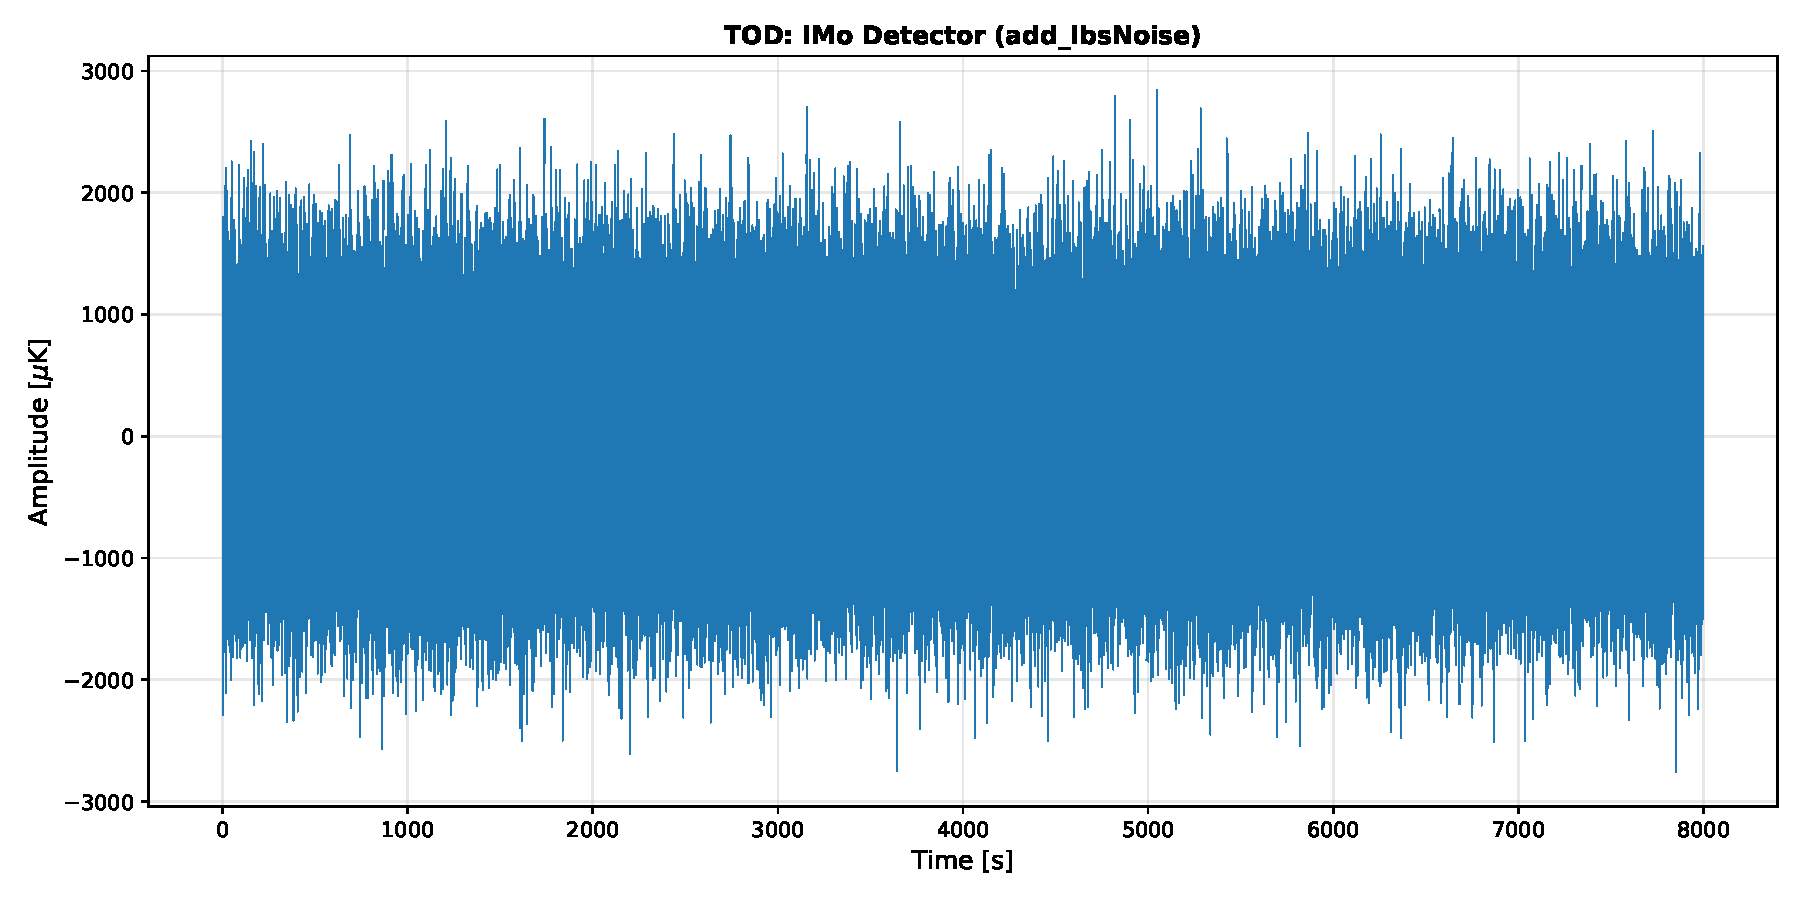
\includegraphics[width=0.68\textwidth]{tod_imo_lbs.pdf}
    \caption{TOD simulated with the IMo detector using \texttt{add\_lbsNoise}.}
    \label{fig:tod_imo_lbs}
\end{figure}

\begin{figure}[h!]
    \centering
    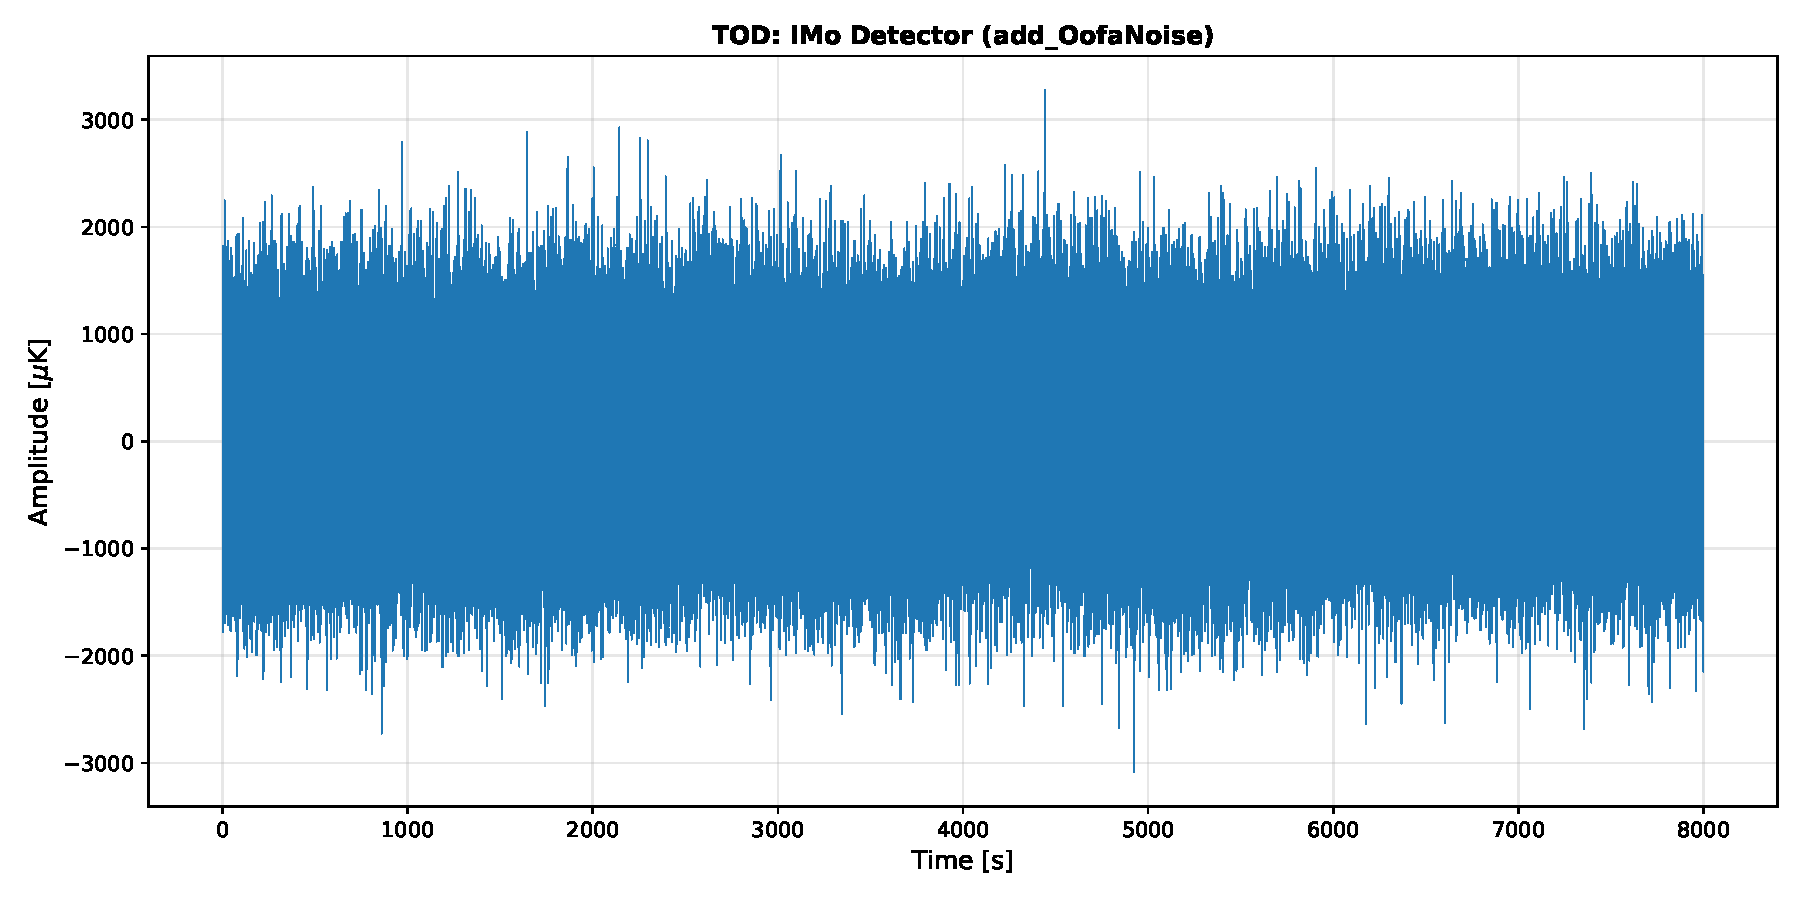
\includegraphics[width=0.68\textwidth]{tod_imo_oofa.pdf}
    \caption{TOD simulated with the IMo detector using \texttt{add\_OofaNoise}.}
    \label{fig:tod_imo_oofa}
\end{figure}

In summary, the time-domain analysis confirms that both models reproduce the expected statistical power and phenomenology of $1/f$ noise, independently of detector choice. The custom detector highlights the $1/f$ behavior over short timescales, while the IMo detector illustrates the dominance of white noise in realistic mission conditions, justifying the need for frequency-domain analysis.




\section{Frequency-Domain Analysis}

After validating the noise models in the time domain, their statistical properties are verified in the frequency domain by comparing the PSD of the simulated TODs with the theoretical model from Chapter~2:

\begin{equation} 
P(f) = \mathrm{NET}^2 \left[ \frac{f^\alpha + f_{knee}^\alpha}{f^\alpha + f_\text{min}^\alpha} \right]. 
\end{equation}  

Spectral analysis clearly separates the white-noise contribution (high frequencies) from the $1/f$ component (low frequencies) and allows verification of the knee frequency $f_\mathrm{knee}$ and spectral index $\alpha$.

The Welch method is adopted to estimate the PSD, reducing variance compared to a simple periodogram. Signals are divided into overlapping segments, windowed with a Hann function, and averaged to obtain a stable spectrum.

For both noise-generation methods and detector types, the Welch parameters are:
\begin{itemize}
    \item Segment length $\text{nperseg}=2^{12}$ samples, yielding a frequency resolution $\Delta f = \frac{\text{nperseg}}{f_{\mathrm{samp}}} \simeq 5$--$7$~mHz for $f_\mathrm{samp}=20$--$31$~Hz, sufficient to resolve the knee and the $1/f$ slope.
    \item $50\%$ overlap to improve averaging without significant computational cost.
    \item Hann window to minimize spectral leakage (the spreading of energy from one frequency to other frequencies) at segment boundaries.
    \item Density scaling in $\mu\mathrm{K}^2/\mathrm{Hz}$.
\end{itemize}

Figures 5.5 and 5.6 show the PSD for the custom detector ($f_{\text{knee}} = 0.5$~Hz, $\mathrm{NET} = 50~\mu\text{K}\sqrt{\text{s}}$). At high frequencies ($f > 1$~Hz), both methods converge to the expected white-noise plateau at $\mathrm{NET}^2 = 2500~\mu\text{K}^2/\text{Hz}$. Below the knee frequency, the spectrum follows the $f^{-\alpha}$ behavior, confirming the presence of the correct long-term correlations. The transition between the white-noise regime and the correlated-noise regime occurs at the expected knee frequency, $f_\mathrm{knee} = 0.5$~Hz.

No significant differences between \texttt{add\_lbsNoise} and \texttt{add\_OofaNoise} are observed. These PSDs are computed directly from the TODs analyzed in Section~5.2, ensuring consistency with time-domain observations.

\begin{figure}[h!]
    \centering
    
\includegraphics[width=0.68\textwidth]{psd_mock_lbs.pdf}
    \caption{PSD of the TOD simulated with the custom detector using \texttt{add\_lbsNoise}.}
    \label{fig:psd_custom_lbs}
\end{figure}

\begin{figure}[h!]
    \centering
    
\includegraphics[width=0.68\textwidth]{psd_mock_oofa.pdf}
    \caption{PSD of the TOD simulated with the custom detector using \texttt{add\_OofaNoise}.}
    \label{fig:psd_custom_oofa}
\end{figure}



The analysis was repeated for the IMO detector ($f_{\text{knee}} = 20$~mHz, $\mathrm{NET} = 114.63~\mu\text{K}\sqrt{\text{s}}$). The resulting PSDs highlight a high-frequency plateau stabilizing around $\mathrm{NET}^2 \simeq 1.3 \times 10^4~\mu\text{K}^2/\text{Hz}$. Despite the relatively low knee frequency being close to the spectral resolution limit of the analysis (approximately $7$~mHz), the characteristic $1/f$ rise remains clearly visible in the spectrum, emerging around $0.02$~Hz.

\begin{figure}[h!]
    \centering
    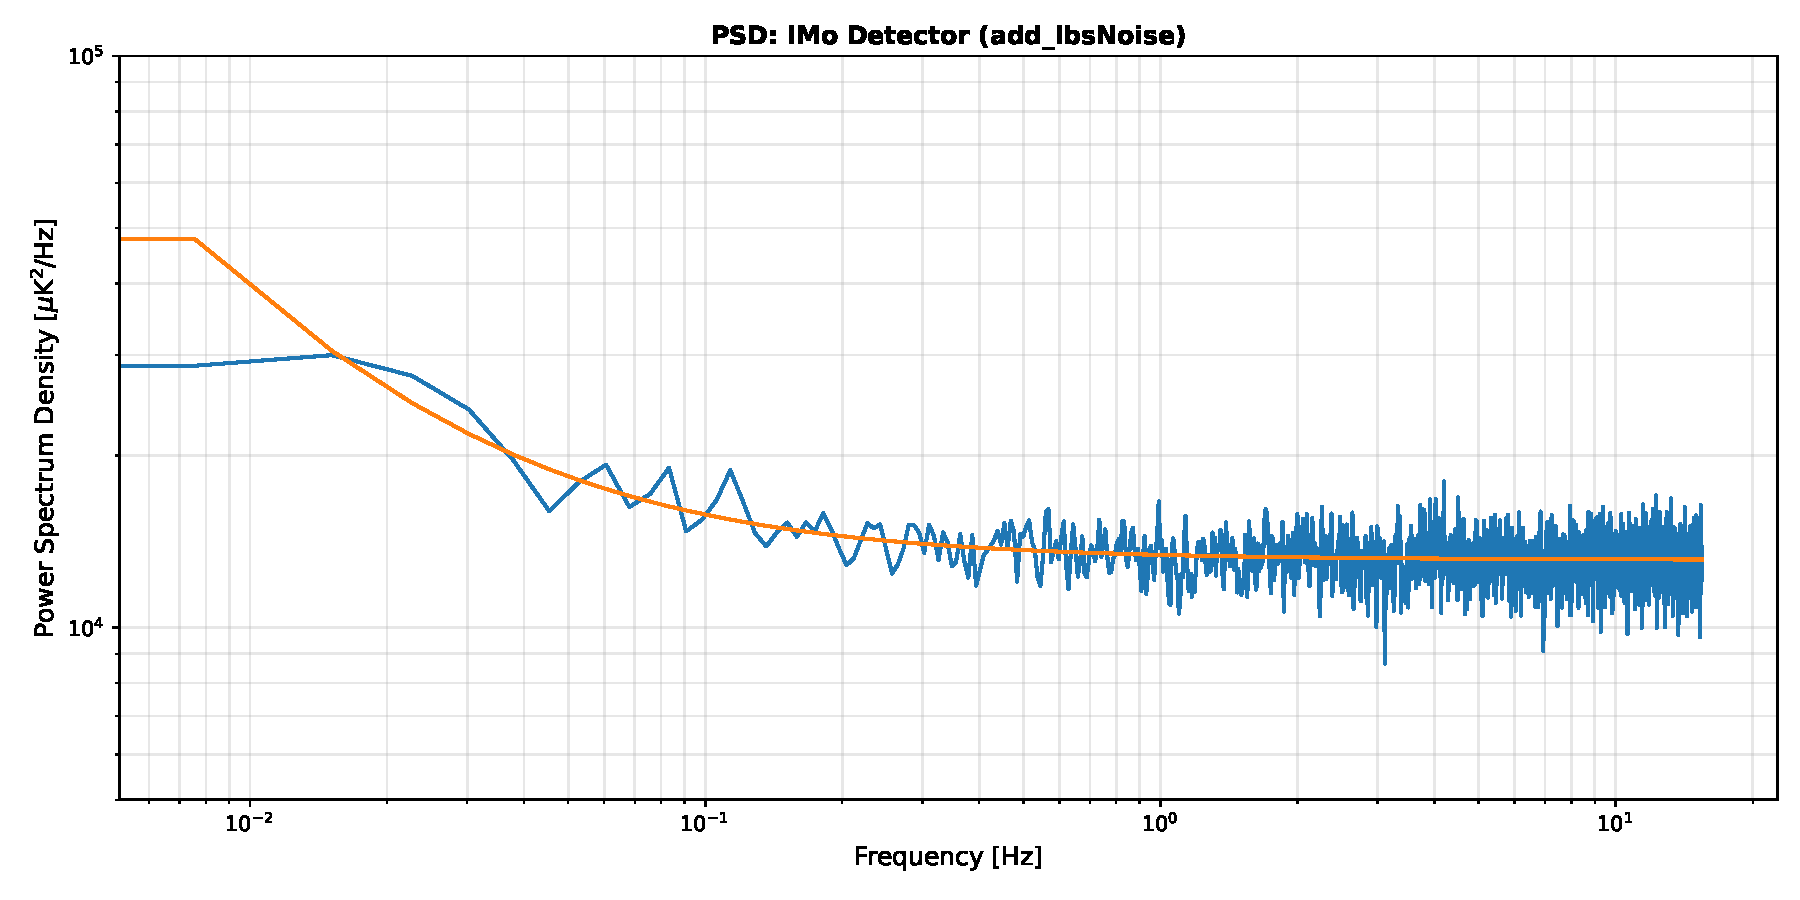
\includegraphics[width=0.68\textwidth]{psd_imo_lbs.pdf}
    \caption{PSD of the TOD simulated with the IMo detector using \texttt{add\_lbsNoise}.}
    \label{fig:psd_imo_lbs}
\end{figure}

\begin{figure}[h!]
    \centering
    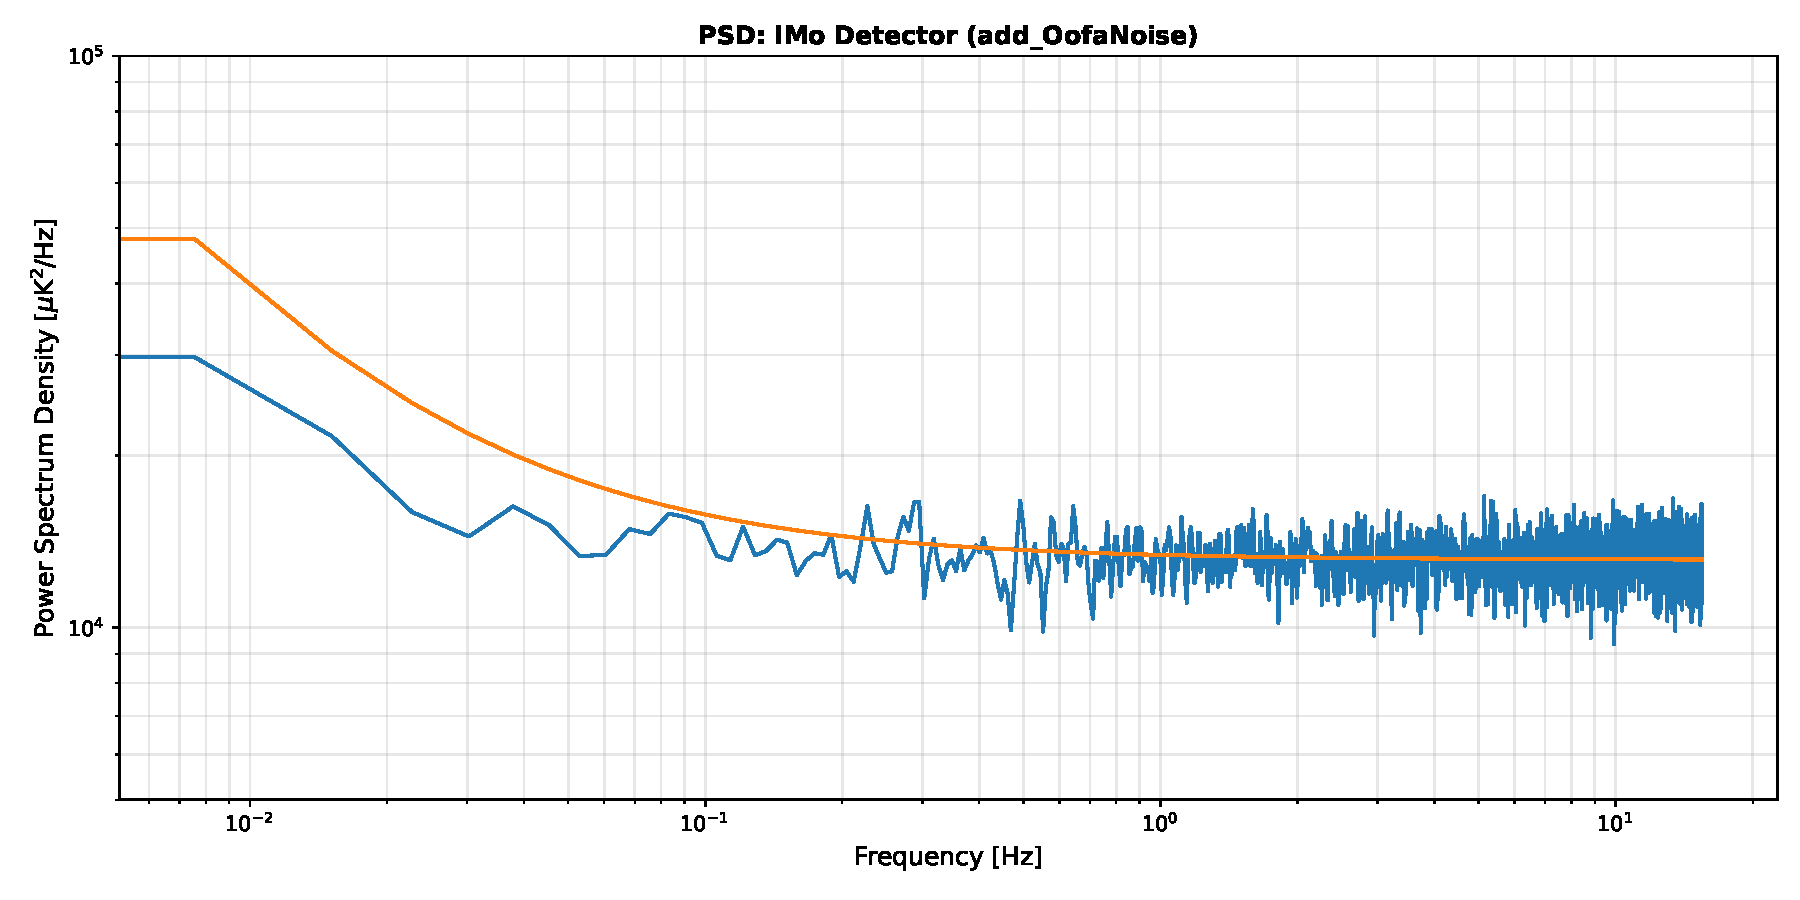
\includegraphics[width=0.68\textwidth]{psd_imo_oofa.pdf}
    \caption{PSD of the TOD simulated with the IMo detector using \texttt{add\_OofaNoise}.}
    \label{fig:psd_imo_oofa}
\end{figure}

These results confirm that both \texttt{add\_lbsNoise} and \texttt{add\_OofaNoise} correctly reproduce the target PSD for both detectors.

Although the comparison in the time and frequency domains provides an initial validation of the noise models, their real impact on cosmological observables only emerges at the map level. For this reason, in the next chapter the analysis is extended to long-duration simulations and to the construction of HEALPix maps.








\chapter{Map-Based Comparison Using HEALPix}

The objective of this chapter is to project the instrumental noise onto the sky by generating noise maps that highlight the spatial manifestation of temporal noise correlations. By implementing a longer simulation, we can examine how $1/f$ drifts translate into systematic patterns on the celestial sphere. Furthermore, this approach allows us to perform an angular power spectrum analysis by decomposing the resulting maps into spherical harmonics.

\section{Long-Term Simulations}

The analysis conducted in Chapter 5 validated the noise models on short timescales ($10^3$~s). However, to evaluate the scientific impact of instrumental noise on cosmological observations, it is necessary to extend the simulation to timescales comparable to the actual mission duration.

$1/f$ noise is intrinsically correlated in time. During scanning operations, the telescope's scanning strategy projects these temporal correlations onto the celestial sphere. While white noise distributes itself uniformly and independently across pixels, the low-frequency fluctuations of correlated noise (drifts) act over long periods, affecting sequences of pixels observed consecutively along the scanning path. This effect typically results in stripes on the final maps.

Only through long-duration simulations can we ensure that the same region of the sky is scanned multiple times with different crossing angles and at different epochs. This process is fundamental for averaging down temporal drifts and ensuring full sky coverage; specifically, a one-year simulation ensures that the scanning strategy covers the entire area of interest with a statistically significant number of hits per pixel.

For this analysis, the setup for the custom detector (summarized in Table 5.1) was maintained. The decision to not use the IMo detector at this stage was driven by the need to emphasize the $1/f$ components. The higher $f_{\text{knee}}$ of the custom model makes the resulting noise patterns more visually and statistically evident in the maps, providing a robust test for the map-making pipeline.

The key parameters for the long-term simulation are:
\begin{itemize}
    \item Total duration: $T_{\text{obs}} = 365$ days ($\approx 3.15 \times 10^7$~s).
    \item Sampling frequency: $f_{\text{samp}} = 20$~Hz.
    \item Total samples: $N_{\text{tot}} = T_{\text{obs}} \cdot f_{\text{samp}} = 630,720,000$.
    \item Noise segmentation: noise generation is divided into 12-hour blocks ($43,200$~s). This scale is sufficiently long to capture all relevant frequencies above $f_{\text{min}}$, while remaining computationally manageable for the generation algorithms.
\end{itemize}

Managing over 600 million samples presents significant computational challenges. Allocating a NumPy array of this size would require approximately 5~GB of RAM for a single detector. Considering that a real mission involves thousands of detectors, the standard approach---loading the entire Time-Ordered Data (TOD), processing it, and then projecting it---becomes impractical. Furthermore, performing a Fast Fourier Transform (FFT) on an entire year of data would impose prohibitive memory requirements and execution times.

To overcome these limitations, an incremental map-making pipeline was implemented:
\begin{enumerate}
    \item The total observation time is partitioned into 12-hour chunks.
    \item For each chunk, the pointing sequences and the corresponding noise TOD are generated on-the-fly.
    \item The data are immediately projected onto the HEALPix map, and the TOD samples are subsequently cleared from memory to free up resources.
    \item The final map is obtained at the end of the cycle by normalizing the accumulated signal by the hit count per pixel.
\end{enumerate}




\section{Map-Making Procedure}

The process of projecting data from the time domain to the spatial domain (maps) represents a fundamental stage of the analysis pipeline. In this work, two types of HEALPix maps were produced for each simulation: a hit-map and a noise-only map.

The hit-map is a map of integers where each pixel contains the total number of samples ($N_p$) that fell within its boundaries during the full year of scanning. This map serves as the metric of the observation: it measures sky coverage, identifies frequently observed regions versus those with lower exposure, and is essential for properly normalizing and averaging the time-domain signal. It is important to note that the hit-map is independent of the presence of noise; it depends exclusively on the scanning strategy and the telescope's pointing geometry.

The noise-only maps contain the generated noise signal. No astronomical signals (CMB or foregrounds) were included in these simulations. This choice aims to isolate the instrumental noise contribution exclusively. In a real-world map, $1/f$ noise is blended with CMB anisotropies; by producing noise-only maps, we can directly visualize the texture produced by temporal correlations and quantify the residual uncertainty that would affect scientific data.

For map production, a binned map-making algorithm was employed. In this configuration, the value of a pixel $m(p)$ is calculated as the simple average of all TOD samples falling into that specific pixel:

\begin{equation}
m(p) = \frac{1}{N_p} \sum_{i \in \text{pixel } p} d_i
\end{equation}

where $d_i$ represents a single TOD sample and $N_p$ is the corresponding value in the hit-map for pixel $p$.

The absence of filtering or pre-processing allows the large-scale structures produced by $1/f$ noise to be fully exposed. This is essential for comparing the \texttt{add\_lbsNoise} and \texttt{add\_OofaNoise} models, as a destriping algorithm would likely mask the very differences we aim to analyze.

In a standard cosmological analysis, this procedure would typically be followed by a destriping phase. Destripers are algorithms designed to suppress the stripes caused by $1/f$ drifts. Although the LBS framework includes an implemented destriping module, it was not utilized in this work. The algorithm is extremely demanding in terms of memory and processing power, as it requires solving large linear systems (one equation per pixel or scanning basket), which exceeded the computational resources available for this study.

In the end, the map resolution is determined by the \texttt{nside} parameter. For this work, $N_{\text{side}} = 2^7 = 128$ was chosen, resulting in a total of $196,608$ pixels on the sphere ($N_{\text{pixel}} = 12N_{\text{side}}^2$). While high-resolution studies typically use $N_{\text{side}} = 512$, the choice of a lower value is justified by the fact that at high resolutions, white noise would visually dominate individual pixels, obscuring large-scale correlations. At $N_{\text{side}} = 128$, the characteristic stripes induced by the temporal correlations of $1/f$ noise become clearly distinguishable, facilitating a qualitative and quantitative comparison between the models.




\section{Memory Optimization and Performance}

Projecting a full year of data onto a HEALPix map presents significant computational challenges for standard Python environments. With over 600 million samples to process, the analysis would be restricted to timescales too short to be scientifically meaningful without dedicated optimization.

In Python, iterating through large-scale arrays using standard \texttt{for} loops is notoriously slow. During initial testing without optimization, simulations were limited to a maximum of 60 days of observation. However, 60 days is insufficient to guarantee the complete and uniform sky coverage required by the LiteBIRD scanning strategy.

So the Numba\footnote{\url{https://numba.pydata.org/}} library was employed. By utilizing the \texttt{@njit} (No-Python Just-In-Time) decorator, critical functions are compiled into highly optimized machine code at runtime.

Specifically, two optimized procedures were implemented to operate directly on memory buffers:
\begin{itemize}
    \item Sample Accumulation: this function performs a loop over detectors and time samples. For each time step, it retrieves the corresponding pixel index from the pointing vector and simultaneously updates two maps: it adds the signal value to the accumulation map and increments the counter in the hit-map by one.
    \item Final Normalization: once the processing of all temporal blocks is complete, this procedure iterates through the entire HEALPix map. For every pixel visited at least once (i.e., where the hit-map value is greater than zero), it calculates the average noise value by dividing the accumulated signal by the number of observations ($N_p$).
\end{itemize}

The implementation of these optimized functions enabled the processing of a full year of simulation data. This, in turn, allowed for complete sky coverage, which is essential for investigating the spatial stripping patterns induced by $1/f$ noise.




\section{Analysis of Noise Maps}

This section presents a qualitative analysis of the HEALPix maps generated by the two noise models: \texttt{add\_lbsNoise} (Figure 6.1) and \texttt{add\_OofaNoise} (Figure 6.2). 

The resulting maps reveal an overlap of two distinct morphological patterns:
\begin{itemize}
    \item Fine-grained fluctuations (White Noise): an isotropic, small-scale random fluctuation is visible in the background. This represents the white noise contribution, which lacks spatial correlations and is distributed independently across pixels.
    \item Striations ($1/f$ Noise): superimposed on the fine-grained background, clear stripes emerge. These striations are the characteristic signature of $1/f$ noise; since the noise is temporally correlated, pixels observed consecutively along the telescope's line of sight tend to share similar values (consistently higher or lower than the mean), creating coherent large-scale structures.
\end{itemize}

The color scales of the maps provide essential quantitative insights. The hit-map shows a non-uniform coverage, with two high-density horizontal bands (peaking at approximately $8,894$ hits per pixel) where the scanning strategy focuses most frequently. In the noise maps, the values are on the order of $10^{-5}$~K (tens of $\mu\text{K}_{\text{CMB}}$), confirming that the noise amplitude is consistent with the detector's NET. The distribution is nearly symmetric around zero, indicating that the generated noise correctly fluctuates without a systematic bias.

A comparison between the \texttt{add\_lbsNoise} and \texttt{add\_OofaNoise} maps reveals strong statistical consistency. Both models faithfully reproduce the same striation texture, and the ranges of minimum and maximum values are remarkably similar. This demonstrates that despite different internal implementations, the total noise power and its projection onto the sphere are correctly preserved by both methods. 

\begin{figure}[h!]
    \centering
    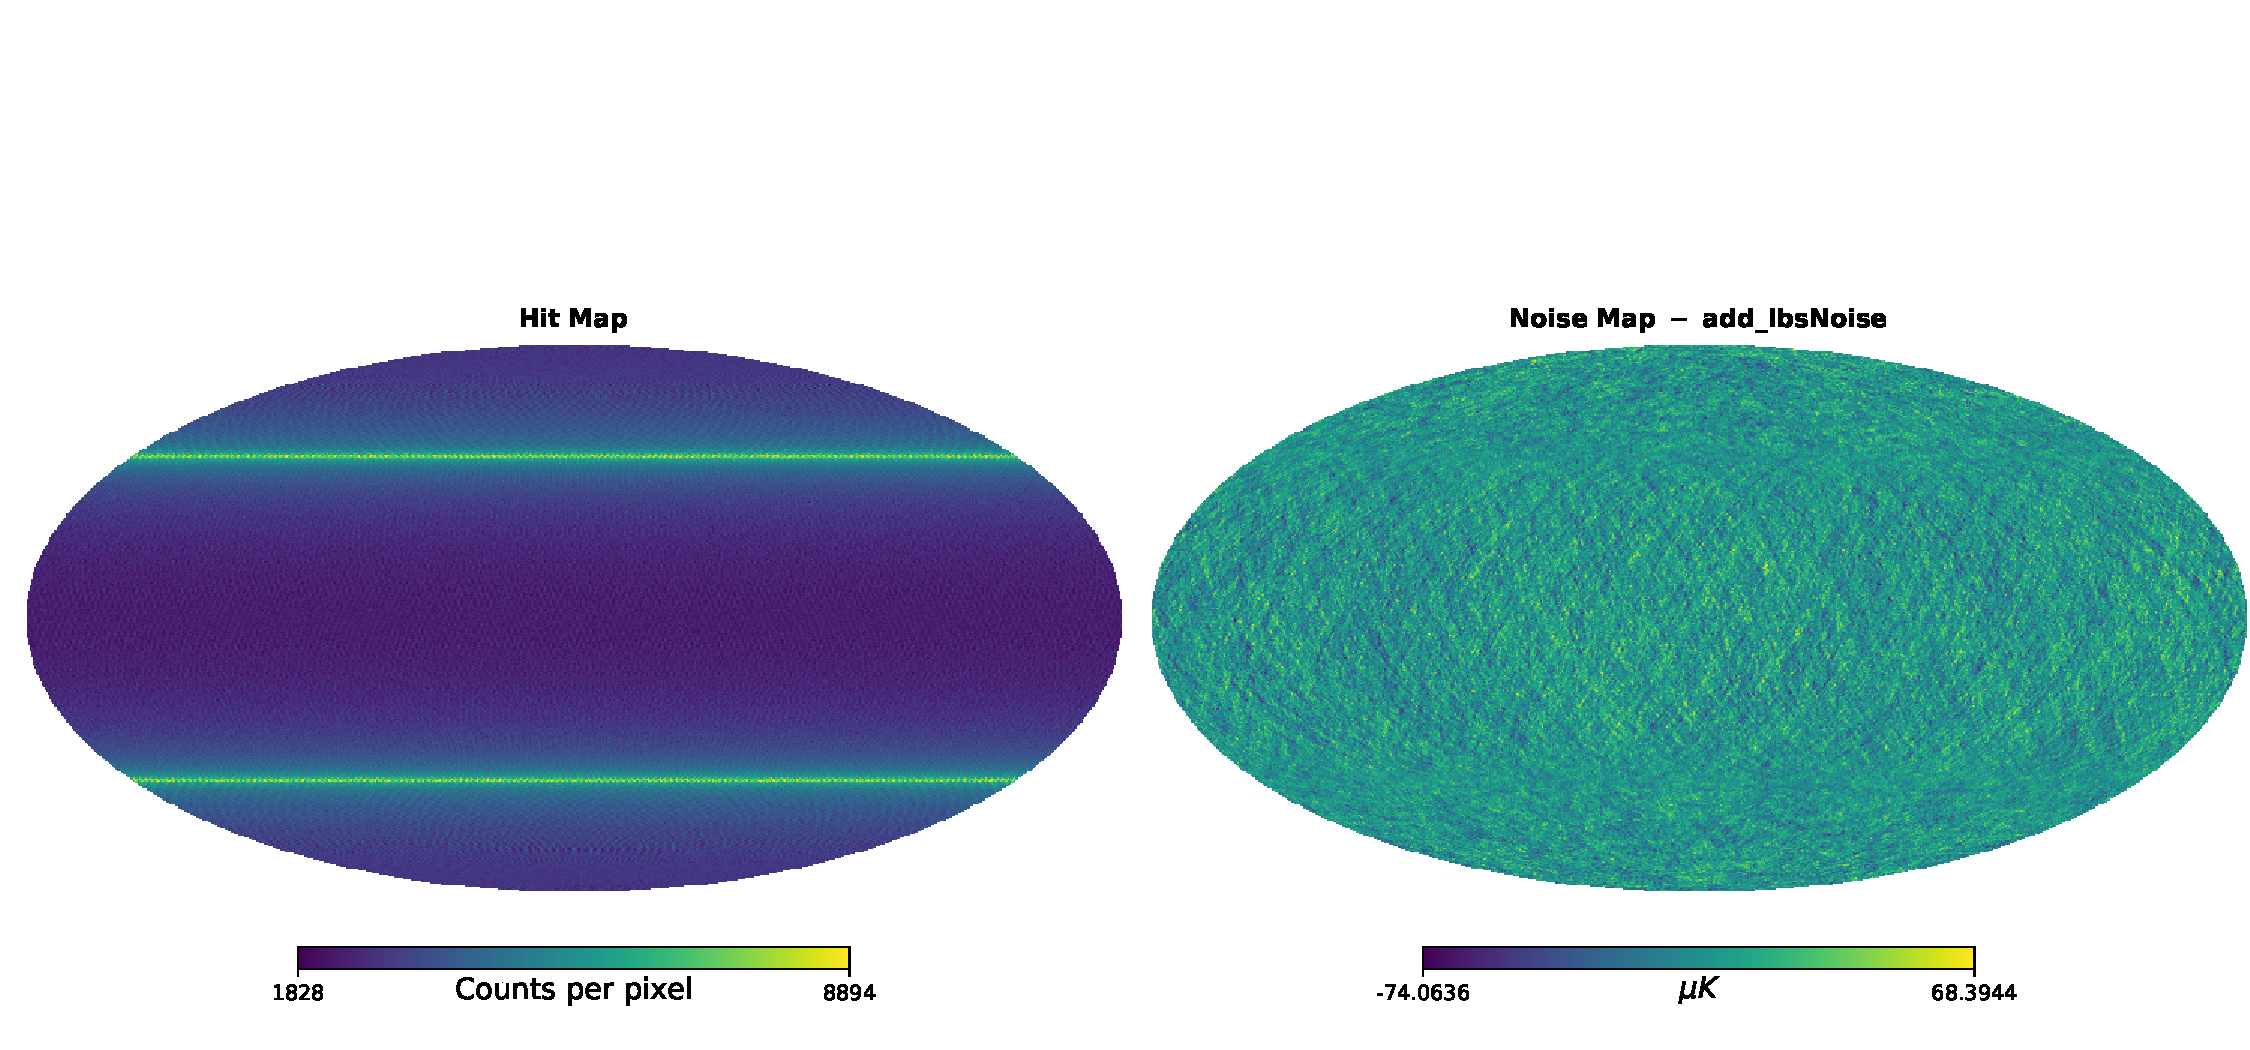
\includegraphics[width=0.8\textwidth]{map_lbs.pdf}
    \caption{HEALPix map using \texttt{add\_lbsNoise}.}
    \label{fig:map_lbs}
\end{figure}

\begin{figure}[h!]
    \centering
    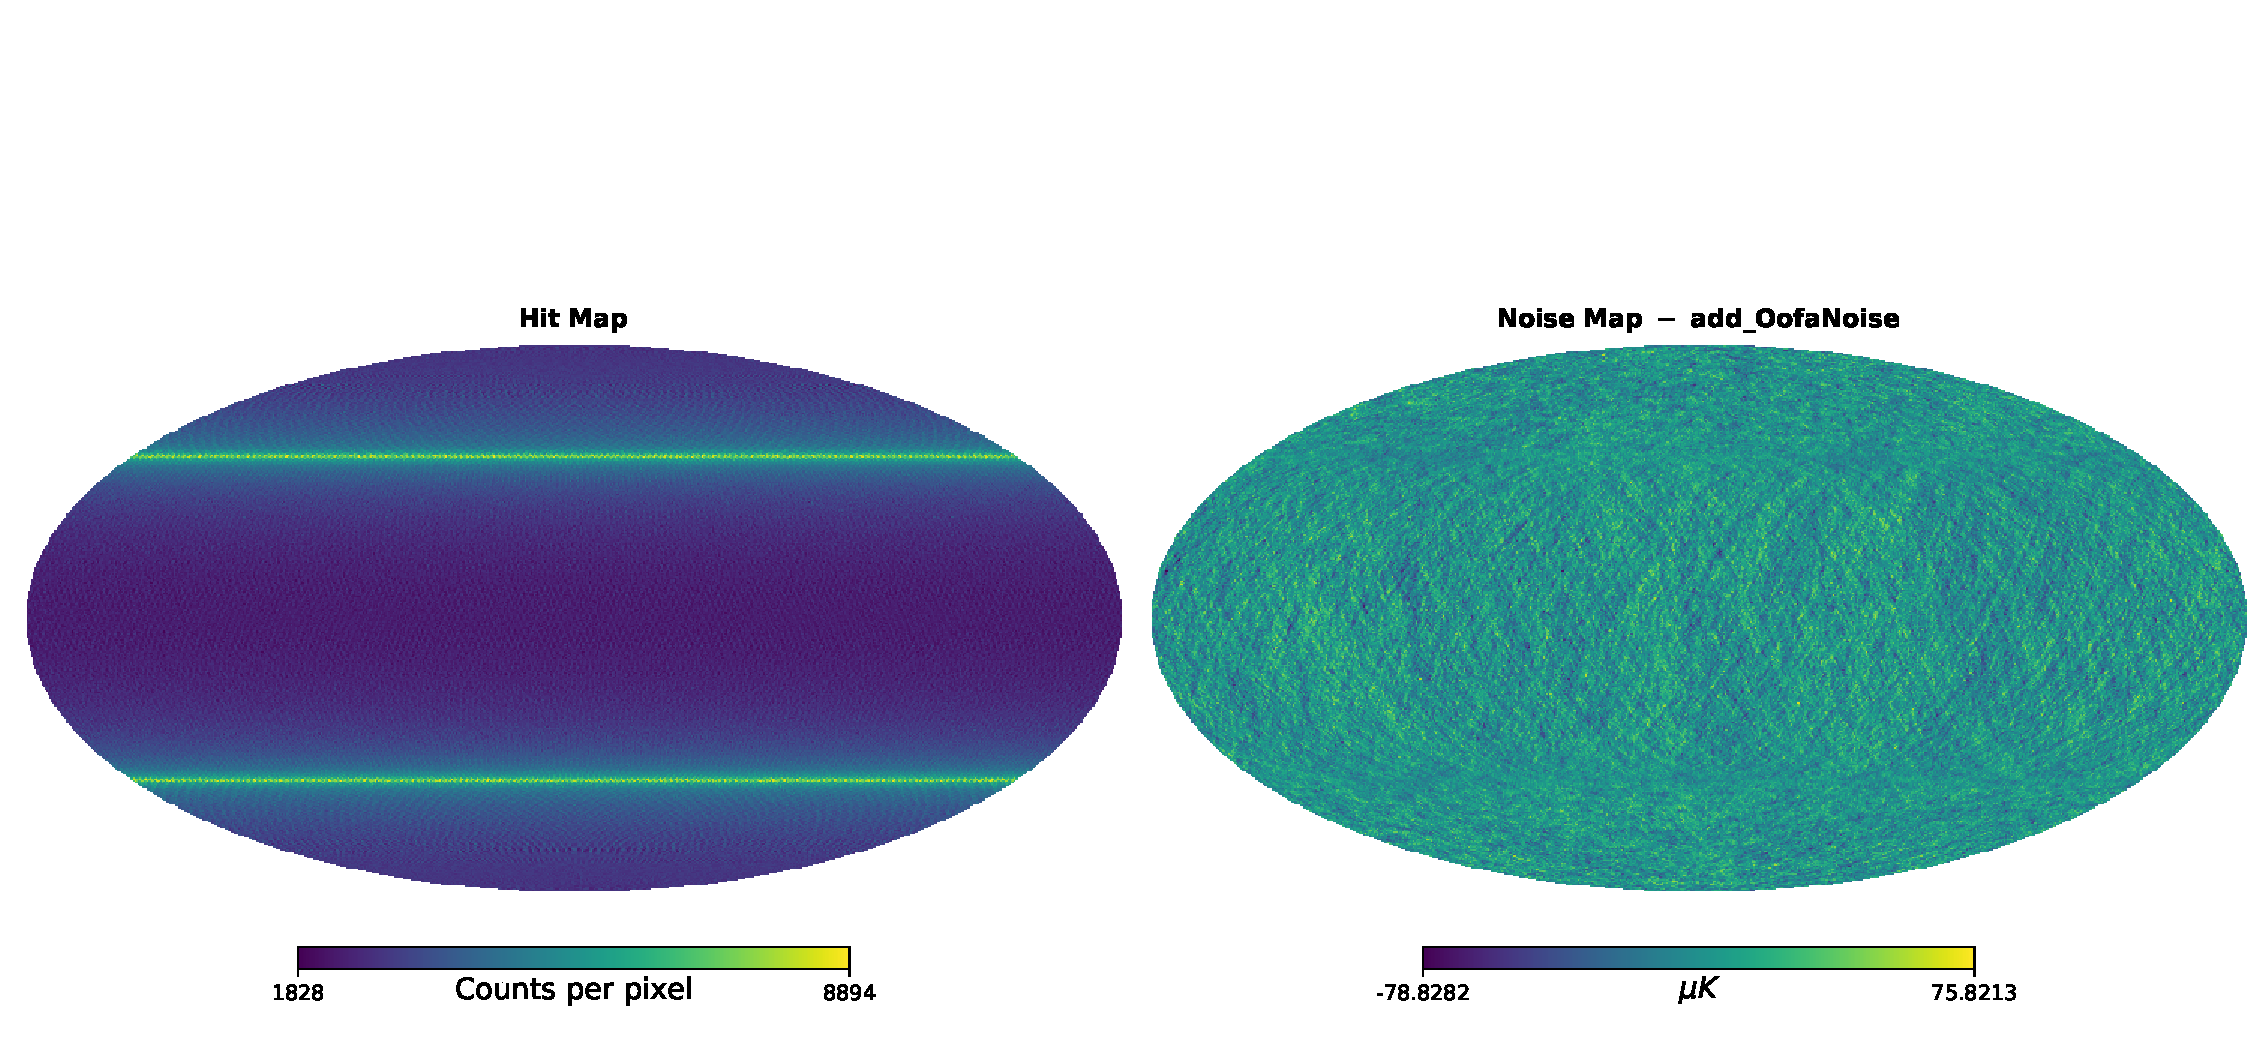
\includegraphics[width=0.8\textwidth]{map_oofa.pdf}
    \caption{HEALPix using \texttt{add\_OofaNoise}.}
    \label{fig:map_oofa}
\end{figure}

An interesting observation concerns the noise uniformity across the celestial sphere. While striations are visible globally, the noise pattern appears more blurred or attenuated in regions frequently visited by the satellite (the brighter bands in the hit-map). This phenomenon is a direct consequence of LiteBIRD's scanning redundancy. When a pixel is observed a high number of times, there is a statistical cancellation of drifts. Different scanning segments crossing the same pixel at distant intervals carry independent noise drifts. 

However, it is important to distinguish the behavior of correlated noise from that of white noise. For a pure white noise signal with a standard deviation in the TOD of $\sigma \approx 220~\mu\text{K}$, a one-year integration (corresponding to approximately $3200$ hits per pixel at $N_{\text{side}}=128$) would reduce the residual noise to $\sigma/\sqrt{N_p} \approx 4~\mu\text{K}$. In contrast, the noise maps generated in this work exhibit fluctuations on the order of tens of $\mu\text{K}$.

This demonstrates that $1/f$ noise does not average down as efficiently as white noise. Because $1/f$ fluctuations possess long-term correlations, the drifts do not cancel out completely even with high redundancy; instead, they leave a residual systematic signal that remains significantly higher than the theoretical white noise limit. This confirms that, while the geometric structure of the scanning strategy acts as a primary natural filter for correlated noise, it cannot fully substitute for dedicated numerical destriping algorithms in preserving the scientific integrity of the maps.

Conversely, in low-density regions where the satellite makes fewer passes, the contrast of individual stripes remains sharp, making the $1/f$ noise much more prominent. This confirms that, even in the absence of numerical destriping algorithms, the geometric structure of the scanning strategy itself acts as a primary, natural filter for correlated noise.




\section{Harmonic-Domain Analysis of Noise Maps}

The final characterization of the noise is conducted in the harmonic domain. This step is essential to quantify the impact of temporal correlations across different angular scales and to statistically validate the consistency between the implemented noise models.

Since the detectors simulated in this work are configured to measure total intensity only, the analysis is restricted to temperature maps ($T$). The spatial domain signal $m(\hat{n})$ is decomposed into the spherical harmonics basis $Y_{\ell m}(\hat{n})$:

\begin{equation}
m(\hat{n}) = \sum_{\ell=0}^{\ell_{\text{max}}} \sum_{m=-\ell}^{\ell} a_{\ell m} Y_{\ell m}(\hat{n})
\end{equation}

From the resulting amplitudes $a_{\ell m}$, the auto-correlated angular power spectrum ($TT$) is calculated:

\begin{equation}
C_\ell^{TT} = \frac{1}{2\ell+1} \sum_{m=-\ell}^{\ell} |a_{\ell m}|^2
\end{equation}

This quantity represents the noise power as a function of the multipole $\ell$, where low $\ell$ values correspond to large angular scales and high $\ell$ values to small angular scales. It should be noted that computing cross-polarized spectra ($EE, BB$) or cross-correlations ($TE$) would require defining the polarization angle for each detector.

A crucial aspect for the validation of this work is the correspondence between the Power Spectral Density in the time domain and the angular power spectrum ($C_\ell$) on the sphere. When generating a map containing only white and $1/f$ noise, the $C_\ell$ trend mirrors the Time-Ordered Data (TOD) properties according to the relation:

\begin{equation}
C_\ell \propto \sigma^2 \left[ 1 + \left( \frac{\ell_{\text{knee}}}{\ell} \right)^\alpha \right]
\end{equation}

In this expression, $\ell_{\text{knee}}$ represents the knee multipole, the spatial equivalent of the temporal knee frequency ($f_{\text{knee}}$). This similarity is not accidental; it reflects how the scanning strategy projects the detector's temporal fluctuations onto the angular scales of the sky. 

For this analysis, we set $\ell_{\text{max}} = 3N_{\text{side}} - 1 = 383$. The choice of $N_{\text{side}}=128$ determines the angular resolution of the map, resulting in a pixel size of approximately $27.5'$, or just under half a degree. Given that the angular scale $\theta$ is approximately related to the multipole by $\ell \approx 180^\circ / \theta$, $\ell \approx 180$ corresponds to degree scales. With the current resolution, the spectrum is reliable up to $\ell \approx 350$.

\begin{figure}[h!]
    \centering
    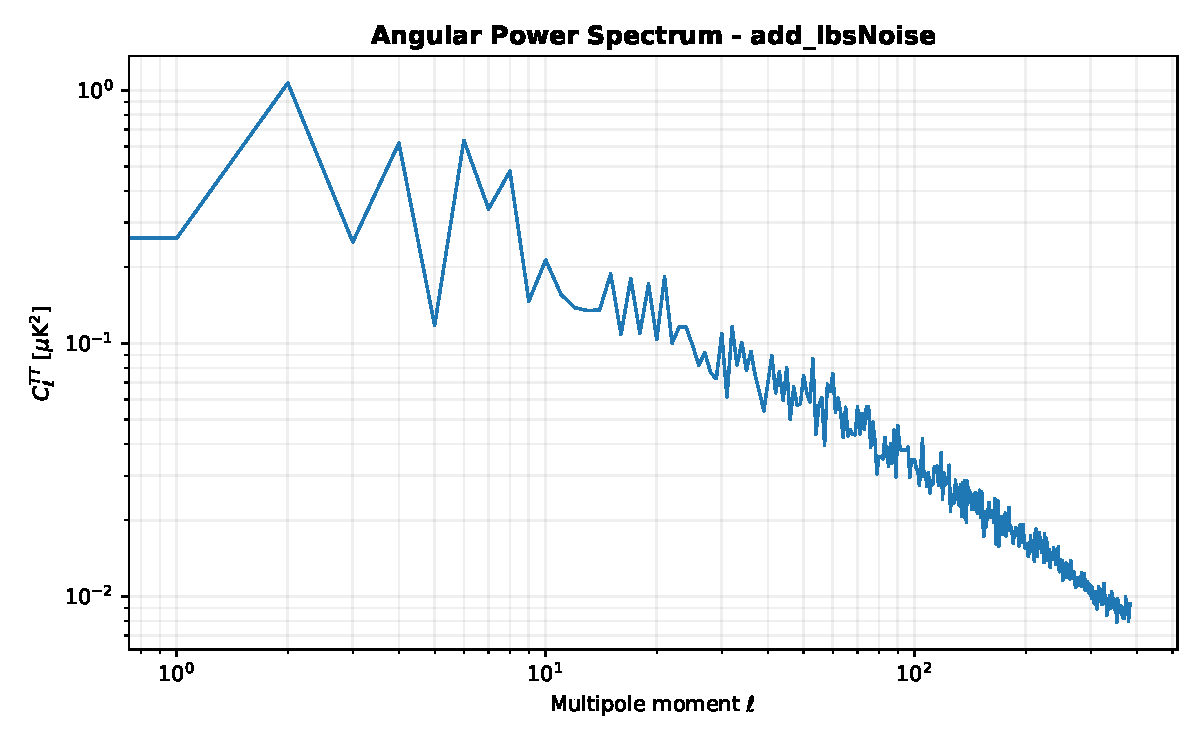
\includegraphics[width=0.65\textwidth]{psd_sh_lbs.pdf}
    \caption{Angular power spectrum using \texttt{add\_lbsNoise}.}
    \label{fig:psd_sh_lbs}
\end{figure}

\begin{figure}[h!]
    \centering
    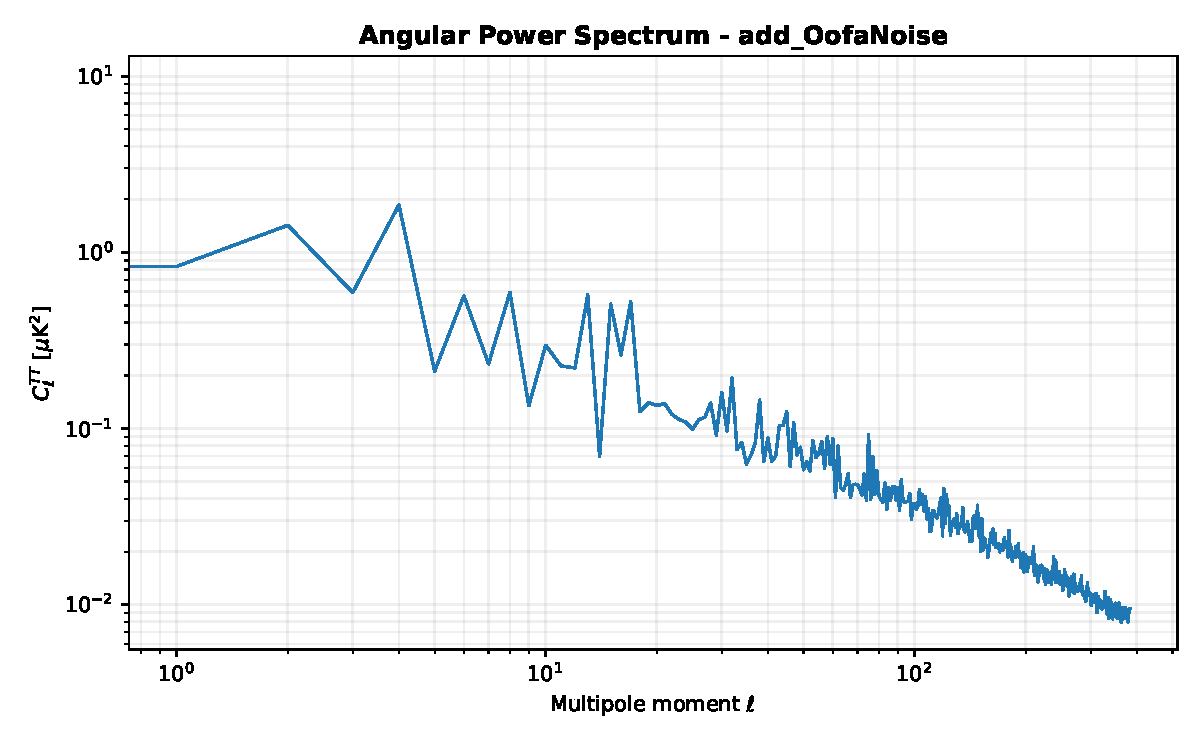
\includegraphics[width=0.65\textwidth]{psd_sh_oofa.pdf}
    \caption{Angular power spectrum using \texttt{add\_OofaNoise}.}
    \label{fig:psd_sh_oofa}
\end{figure}

The power spectra obtained for \texttt{add\_lbsNoise} (Figure 6.3) and \texttt{add\_OofaNoise} (Figure 6.4) exhibit very similar behaviors. Two main features emerge:
\begin{itemize}
    \item Low-$\ell$ Power Excess: both spectra show a marked descending slope at low multipoles. This is the signature of $1/f$ noise: long-term temporal correlations translate into large-scale spatial correlations (low multipoles) on the sky.
    \item Absence of a White Noise Plateau: in an ideal or filtered scenario, the spectrum would be expected to flatten into a plateau at high $\ell$, where white noise dominates. However, in these results, the $1/f$ noise is so predominant that it masks the white noise contribution up to the map resolution limit ($\ell \approx 350$).
\end{itemize}

The persistence of this slope is also due to the use of a simple binned map-maker. Had a destriping algorithm been applied, the low-frequency correlated components would have been suppressed, allowing the white noise plateau to emerge clearly in the spectrum. 

The comparison between the power spectra obtained for \texttt{add\_lbsNoise} and \texttt{add\_OofaNoise} reveals a strong statistical consistency between the two generation methods. Both spectra exhibit the same characteristic descending slope at low multipoles and maintain an almost identical power distribution across the entire range of $\ell$. 


\chapter{Conclusions}

\section{Summary of the Work}
In this thesis, we have addressed one of the most critical aspects of Cosmic Microwave Background (CMB) simulations: the modeling and generation of correlated instrumental noise for the LiteBIRD mission. 

The core of this work consisted in the implementation of two independent, block-wise noise-generation functions: \texttt{add\_lbsNoise}, based on the LiteBIRD Simulation framework, and \texttt{add\_OofaNoise}, based on the \texttt{ducc0} library. This development has led the simulation process to move from a monolithic to a segmented approach, memory-efficient pipeline, enabling the simulation of long-duration Time-Ordered Data (TOD) that would otherwise be computationally prohibitive.

The models were validated through a different testing strategy:
\begin{itemize}
    \item Time and Frequency Domains: short-term simulations confirmed that both methods accurately reproduce the target $1/f$ Power Spectral Density (PSD).
    \item Map Domain: long-term simulations were performed using a JIT-optimized (Numba) map-making pipeline. These tests allowed us to visualize the spatial stripping patterns caused by temporal correlations and to confirm that the scanning strategy's redundancy naturally mitigates $1/f$ drifts. Furthermore, the generated maps enabled the calculation of the angular power spectrum ($C_\ell^{TT}$).
\end{itemize}




\section{Final Comparison Between Noise Models}
The comparison between the two implemented approaches are summarized in Table~7.1.

\begin{table}[h!]
\centering
\begin{tabular}{lll}
\toprule
\textbf{Feature} & \textbf{add\_lbsNoise (FFT-based)} & \textbf{add\_OofaNoise (Filter-based)} \\ \midrule
Implementation & FFT-based stochastic generation & Recursive digital filtering \\
Memory Usage & Scalable with block size & Minimal and constant \\
Continuity & Potential block-edge jumps & Intrinsic temporal continuity \\
Spectral Flexibility & High (arbitrary PSDs) & Rigid (fixed $1/f^\alpha$ model) \\
Integration & Native to LBS & Requires parameter conversion \\
Performance & Efficient for medium blocks & Superior for long durations \\ \bottomrule
\end{tabular}
\caption{Comparative analysis between the LBS and ducc0-based noise generation functions.}
\label{tab:comparison_models}
\end{table}

While \texttt{add\_lbsNoise} remains a versatile tool for simulating complex, non-standard noise spectra, \texttt{add\_OofaNoise} proved to be a more robust solution. Its key advantages reside in its ability to maintain perfect continuity across block boundaries and its significantly lower memory footprint. Additionally, the \texttt{ducc0} implementation demonstrated a slight performance advantage, reducing execution times by a margin ranging from a few seconds up to one minute for the longest simulations in this work.



\section{Future Improvements}
The framework developed in this thesis provides a solid foundation for more complex simulation scenarios. Future developments could include:

\begin{itemize}
    \item Multi-Detector Correlations: extending the block-wise functions to handle multi-detector arrays where individual detectors are characterized by different noise parameters.
    \item Signal-plus-Noise Pipelines: integrating the noise models with actual CMB anisotropies and Galactic foreground signals to test the effectiveness of destriping algorithms in recovering the cosmological signal.
\end{itemize}

In conclusion, this work demonstrates that a block-wise approach to noise generation is a computational necessity for modern CMB experiments.





\cleardoublepage
\printbibliography

% ====== APPENDICI ======
\cleardoublepage
\appendix
\renewcommand{\thechapter}{\Alph{chapter}} 


% Carica il file unico
\chapter{Implementation Details and Simulation Code}
\label{appendix:code}

This appendix provides the Python implementation of the main components of this thesis. The code is organized into three main sections: time and frequency domain validation (Chapter 5), the map-making and harmonic analysis pipeline (Chapter 6), and functions optimized using Just-In-Time (JIT).

\section{Time and Frequency Domain Analysis}
This script handles noise model validation by producing simulated time-ordered data (TOD) and the theoretical power spectral density (PSD) model. Although the following code uses a "mock detector" for demonstration, a real detector can be loaded from the LiteBIRD instrument model (IMo).

\begin{lstlisting}[language=Python, caption={Validation of noise statistics in time and frequency domains.}]
import litebird_sim as lbs
import numpy as np
from scipy.signal import welch
from mylib import add_lbsNoise, add_OofaNoise

# --- Simulation Setup ---
start_time = 0
time_span_s = 1000.0  # Duration sufficient for 1/f characterization

sim = lbs.Simulation(
    start_time=start_time,
    duration_s=time_span_s,
    random_seed=12345,
    imo=lbs.Imo(flatfile_location=lbs.PTEP_IMO_LOCATION)
)

# --- Scanning Strategy ---
sim.set_scanning_strategy(
    lbs.SpinningScanningStrategy(
        spin_sun_angle_rad=np.deg2rad(0),
        precession_rate_hz=0,
        spin_rate_hz=1/60,
        start_time=start_time,
    ),
    delta_time_s=5.0,
)

# --- Detector Setup ---
# Note: Parameters can be substituted with IMO data 
det = lbs.DetectorInfo(
    name="Boresight_detector",
    sampling_rate_hz=20.0,
    bandcenter_ghz=100.0,
    net_ukrts=50.0,
    fknee_mhz=500.0,
    fmin_hz=1e-5,
    alpha=1.0
)

sim.create_observations(detectors=det)
tod = sim.observations[0].tod 

# --- Noise Generation ---
# Model selection: add_lbsNoise (FFT-based) or add_OofaNoise (Filter-based)
add_lbsNoise(tod, det, block_duration_s=100)

# --- Spectral Estimation (Welch Method) ---
frequencies, psd = welch(
    tod,
    fs=det.sampling_rate_hz,
    window='hann',
    nperseg=2**12,
    noverlap=2**11,
    scaling='density',
    return_onesided=False
)

# Sorting frequencies for analysis
sort_idx = np.argsort(frequencies)
frequencies = frequencies[sort_idx]
psd = psd[:, sort_idx]

# --- Theoretical PSD Comparison ---
f = frequencies
f_knee = det.fknee_mhz / 1000.0  # Convert to Hz
f_min = det.fmin_hz

# Analytical model for 1/f + white noise
theoretical_psd = (det.net_ukrts**2) * ( (f**det.alpha + f_knee**det.alpha) / (f**det.alpha + f_min**det.alpha) )
\end{lstlisting}





\section{Full Map-Making and Harmonic Analysis Pipeline}
This section presents the integrated pipeline used to generate the long-term simulation results discussed in Chapter 6. The implementation adopts an incremental map-making strategy to maintain a minimal memory footprint by processing 365 days of observation in 12-hour chunks. 

The final part of the script illustrates the harmonic decomposition of the resulting noise maps to estimate the angular power spectrum $C_\ell^{TT}$.

\begin{lstlisting}[language=Python, caption={Incremental map-making and angular power spectrum estimation.}]
import healpy as hp
import numpy as np
from uuid import UUID
import litebird_sim as lbs
from mylib import add_OofaNoise, add_lbsNoise, add_samples_to_map, normalize_map

# --- 1. Simulation & Instrument Configuration ---
nside = 128  # Map resolution
lmax = 3 * nside - 1
chunk_length = 3600 * 12  # 12-hour blocks
number_of_days = 365
duration_s = 86400 * number_of_days 
num_of_observations = duration_s // chunk_length

sim = lbs.Simulation(
    start_time=0,
    duration_s=duration_s,
    random_seed=12345,
    imo=lbs.Imo(flatfile_location=lbs.PTEP_IMO_LOCATION)
)

# Scanning Strategy (LiteBIRD Spinning Strategy)
sim.set_scanning_strategy(
    lbs.SpinningScanningStrategy.from_imo(
        imo=lbs.Imo(lbs.PTEP_IMO_LOCATION), 
        url=UUID("117fd641-a925-4eeb-9fda-f7c468682108")
    ),
    delta_time_s=120.0
)

# Instrument and Detector Setup
instrument = lbs.InstrumentInfo(
    boresight_rotangle_rad=0.0,
    spin_boresight_angle_rad=np.deg2rad(90),
    spin_rotangle_rad=np.deg2rad(75)
)
sim.set_instrument(instrument)

det = lbs.DetectorInfo(
    name="Boresight_detector", sampling_rate_hz=20.0, net_ukrts=50.0,
    fknee_mhz=500.0, fmin_hz=1e-5, alpha=1.0
)

# --- 2. Incremental Processing Loop ---
# Allocate metadata without full TOD arrays to save RAM
sim.create_observations(detectors=det, num_of_obs_per_detector=num_of_observations, allocate_tod=False)

# Pre-allocate map buffers and temporary TOD block
accum_map = np.zeros(hp.nside2npix(nside))
hit_count_map = np.zeros(len(accum_map), dtype='int64')
tod_buffer = np.empty((1, int(det.sampling_rate_hz * chunk_length)))

for obs_idx, cur_obs in enumerate(sim.observations):
    # A. Pointing Generation
    lbs.prepare_pointings(cur_obs, instrument, sim.spin2ecliptic_quats)
    pointings, _ = cur_obs.get_pointings("all")
    pixidx = hp.ang2pix(nside, pointings[0,:,0], pointings[0,:,1])
    
    # B. Noise Generation (In-place)
    tod_buffer[:, :] = 0.0
    add_OofaNoise(tod_buffer, det, block_duration_s=chunk_length)
    
    # C. Map Accumulation (using Numba-optimized kernels)
    add_samples_to_map(tod_buffer, pixidx, accum_map, hit_count_map)  

# Final normalization (Binned Map-Making)
normalize_map(accum_map, hit_count_map)

# --- 3. Harmonic Analysis (Power Spectrum Estimation) ---
# The following steps decompose the map into Spherical Harmonics 
# and compute the auto-correlation power spectrum.

almT = hp.map2alm(accum_map, lmax=lmax)
clTT = hp.alm2cl(almT)
\end{lstlisting}





\section{Numba-Optimized Kernels}
These functions are decorated with \texttt{@njit} to handle the high-speed accumulation of TOD samples into HEALPix pixels.

\begin{lstlisting}[language=Python, caption={Performance-critical Numba kernels for sample accumulation and map normalization.}]
from numba import njit

@njit
def add_samples_to_map(tod, pixel_indexes, accum_map, hit_count_map):
    """
    Accumulates TOD samples into the HEALPix maps using JIT-optimized loops.
    
    Parameters:
    - tod: 2D array (ndet, nsample) containing the noise data.
    - pixel_indexes: 1D array of pixel indices corresponding to the scan strategy.
    - accum_map: The map where signal values are summed.
    - hit_count_map: The map counting the number of observations per pixel.
    """
    ndet, nsample = tod.shape

    for det_idx in range(ndet):
        for sample_idx in range(nsample):
            pix_idx = pixel_indexes[sample_idx]
            accum_map[pix_idx] += tod[det_idx, sample_idx]
            hit_count_map[pix_idx] += 1

@njit
def normalize_map(accum_map, hit_count_map):
    """
    Performs binned map-making normalization by dividing the accumulated 
    signal by the hit count.
    """
    for pix_idx in range(len(accum_map)):
        if hit_count_map[pix_idx] > 0:
            accum_map[pix_idx] /= hit_count_map[pix_idx]
\end{lstlisting}



\end{document}


